\chapter{Localisation}
\label{localisation}

% **************************** Define Graphics Path **************************
\graphicspath{{Chapter3/Figs/}}

\section{Introduction}

{\let\thefootnote\relax\footnote{{In this Chapter, \cref{sec:model} and \cref{sec:exp} was collaborative work with Matthew Grimes and Roberto Cipolla and was published in \citep{kendall2015posenet}.}}}

\begin{figure}[t]
	\begin{center}
		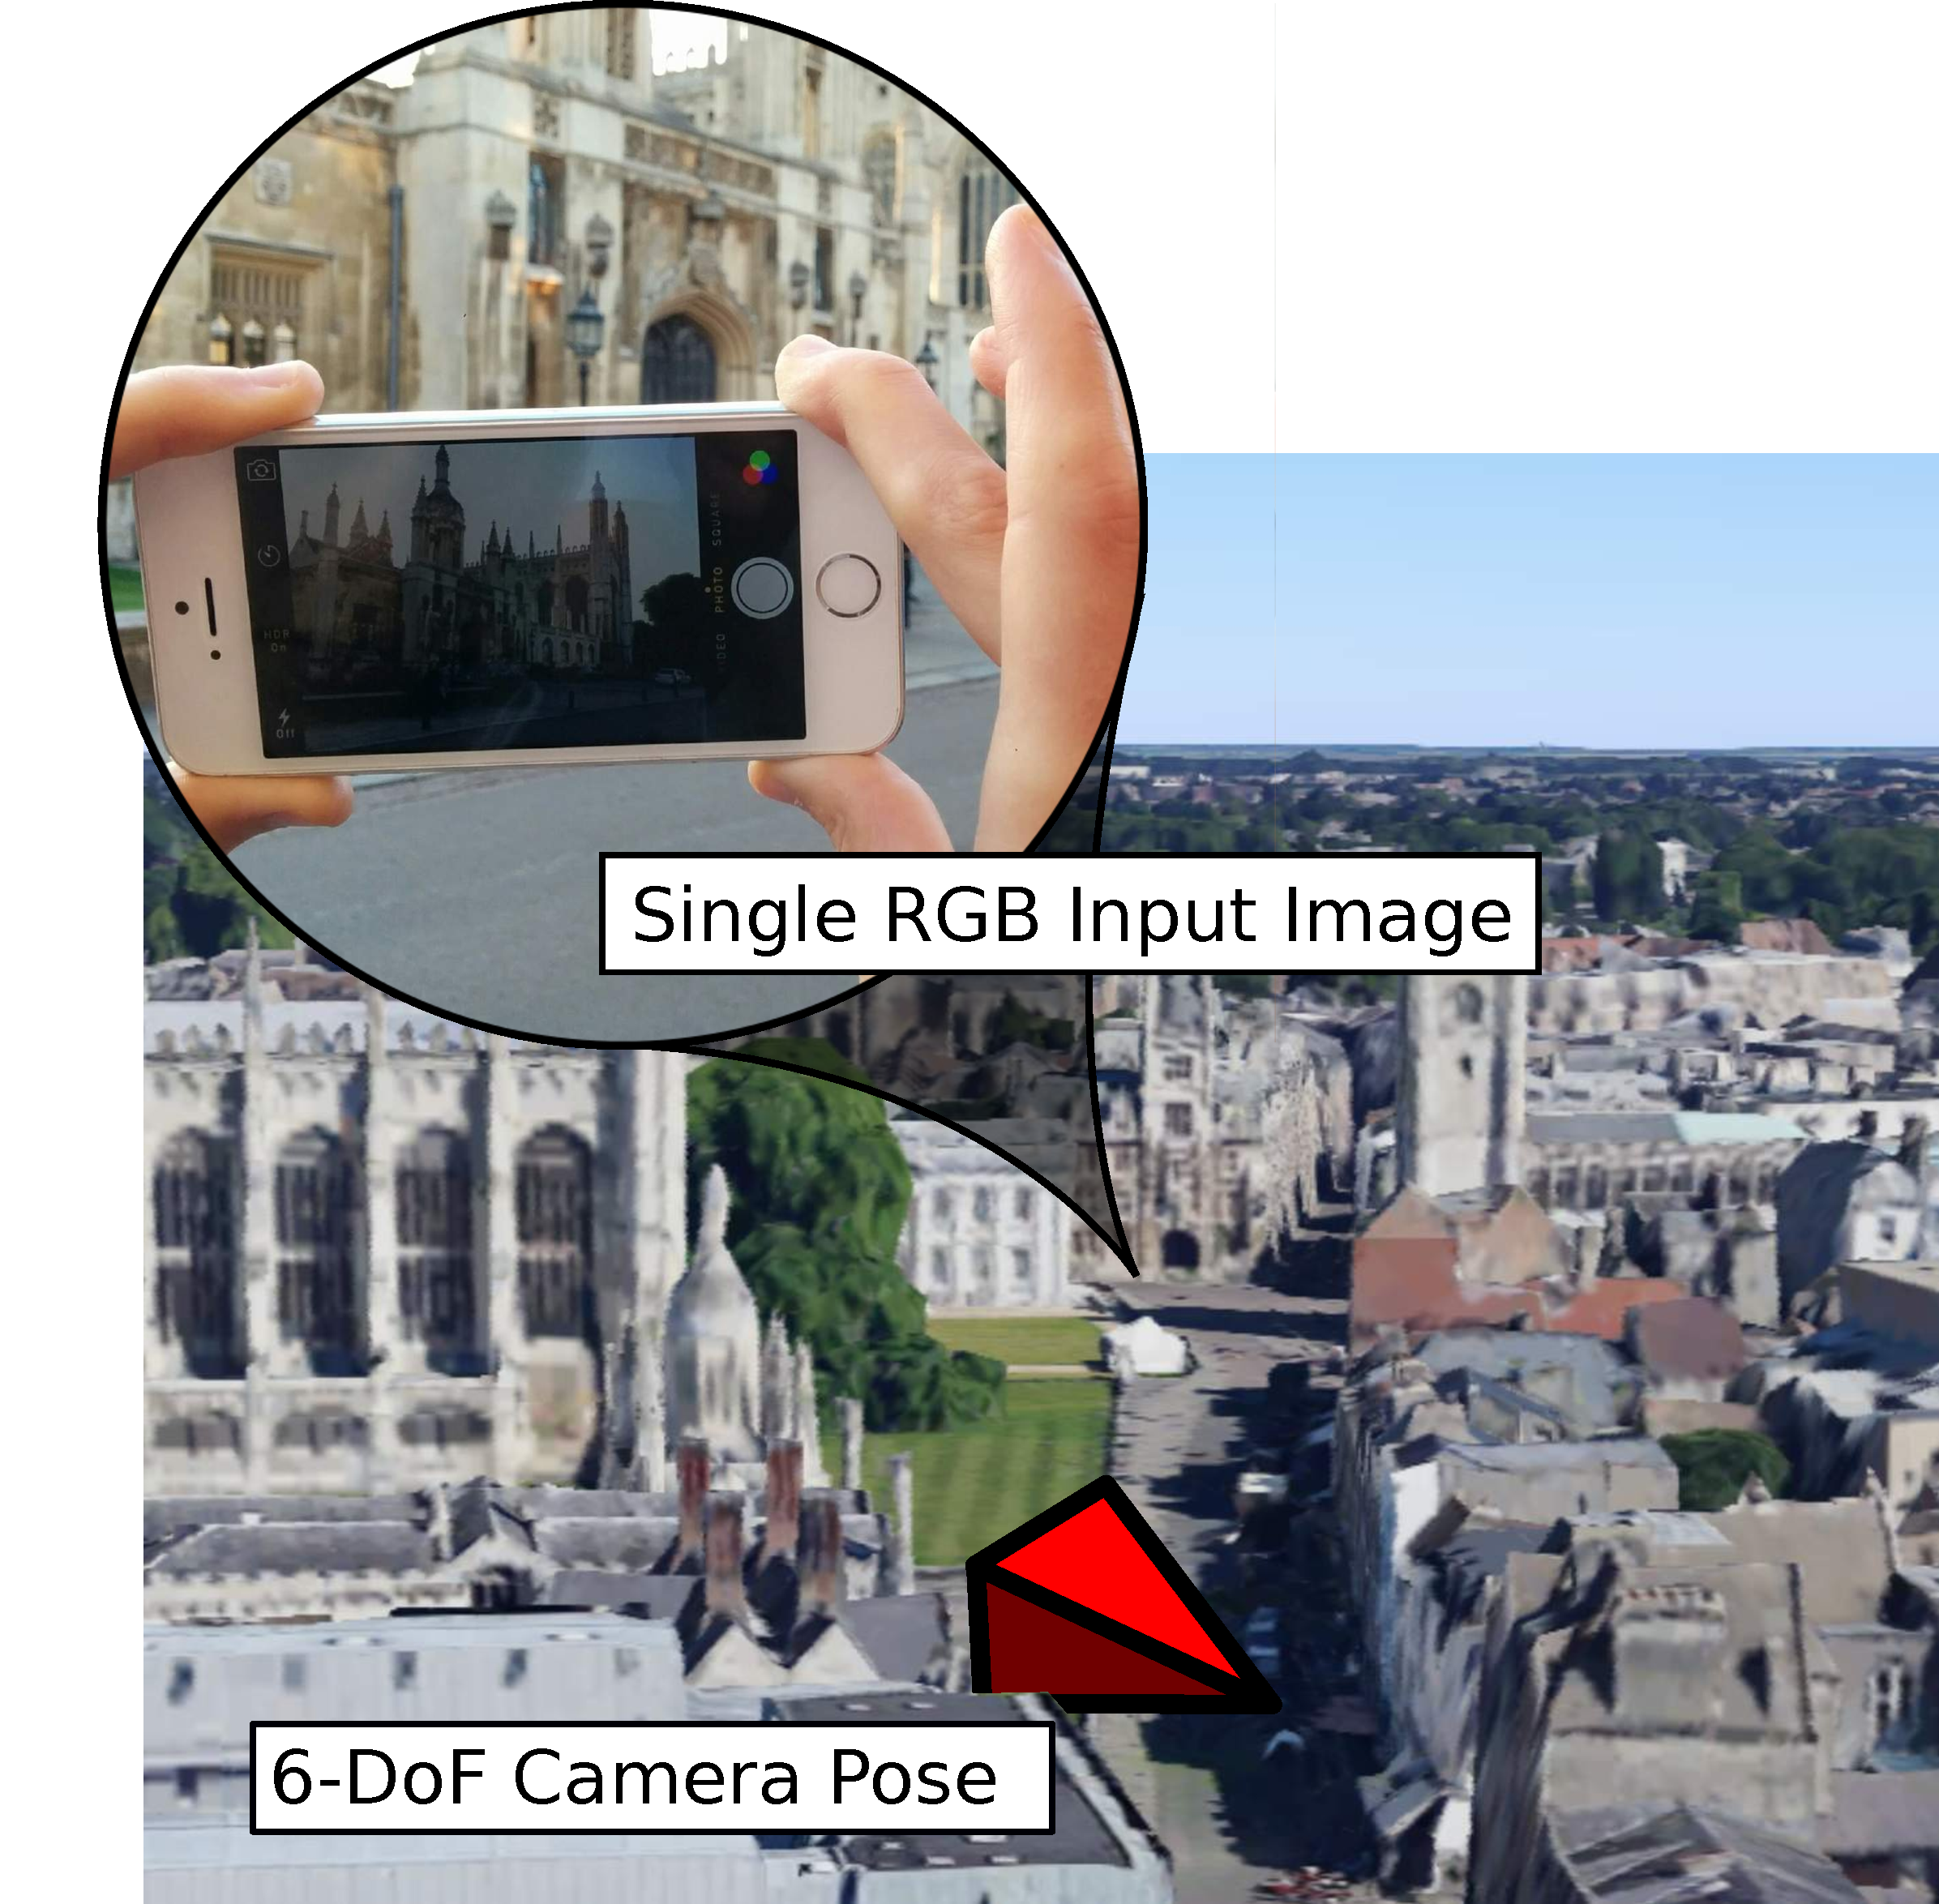
\includegraphics[width=0.5\linewidth]{teaser.pdf}
	\end{center}
	\caption[PoseNet: Convolutional networks for 6-DOF camera pose regression]{\textbf{PoseNet} \citep{kendall2015posenet} is trained end-to-end to estimate the camera's six degree of freedom pose from a single monocular image.}
	\label{teaser}
\end{figure}

In this chapter we address the problem of localisation --- estimating the camera's position and orientation in three-dimensional space. This is also colloquially known as the \textit{kidnapped robot problem} and is essential for many applications including mobile robotics, navigation and augmented reality. 

Designing a system for reliable large scale localisation is a challenging problem. The discovery of the positioning system in mammalian brains, located in the hippocampus, was awarded the 2014 Nobel prize in Physiology or Medicine \citep{o1978hippocampus,moser2008place}. State of the art computer vision localisation systems perform very well within controlled environments \citep{klein2007parallel,newcombe2011dtam,engel2014lsd,mur2015orb,Sattler14ECCV}. However, we are yet to see their wide-spread use in the wild because of their inability to cope with novel viewpoints or large environmental changes.

Many of the visual localisation systems use point landmarks such as corners \citep{robertson2004image}, SIFT \citep{lowe2004distinctive} or ORB \citep{rublee2011orb} to localise. These features perform well for incremental tracking and estimating ego-motion \citep{mur2015orb}. However, point features cannot encode context and are not able to create a representation which is sufficiently robust to challenging real-world scenarios. For example, they often fail under varying weather, lighting or environmental conditions. Additionally, they lack the ability to capture global context and require robust aggregation of hundreds of points to form a consensus to predict pose \citep{zeisl2015camera}.





This chapter proposes a framework which learns to localise from a single image using deep learning. Our localisation system, PoseNet \citep{kendall2015posenet,kendall2015modelling,kendall2017posenet}, takes a single RGB image and regresses the camera's 6-DoF pose relative to a scene. \cref{teaser} illustrates an example. The algorithm is simple in the fact that it consists of a convolutional neural network trained end-to-end to regress the camera's orientation and position. We show that we can localise more robustly using deep learning, compared with point features such as SIFT \citep{lowe2004distinctive}. PoseNet learns a representation using the entire image context based on appearance and shape. These features generalise well and can localise across challenging lighting and appearance changes. It operates in real time, taking 5ms to run, and obtains approximately 2m and 3 degrees accuracy for large scale outdoor scenes (covering a ground area of up to $50,000m^2$). It is very scalable as it does not require a large database of landmarks. Rather, it learns a mapping from pixels to a high dimensional space linear with pose.

We introduce novel techniques and loss functions to design the deep convolutional neural network camera pose regressor. We leverage transfer learning from recognition to relocalisation with very large scale classification datasets. Additionally we use structure from motion to automatically generate training labels (camera poses) from a video of the scene. This reduces the human labour in creating labelled video datasets to just recording the video. We show that the system learns to compute feature vectors which are easily mapped to pose, and which also generalize to unseen scenes with a few additional training samples.

The remainder of the chapter discusses two improvements to PoseNet, using \textit{geometry} and \textit{uncertainty}.

The main weakness of PoseNet in its initial form was that, despite its scalability and robustness, it does not produce metric accuracy which is comparable to other geometric methods \citep{Sattler14ECCV,svarm2014accurate}. We argue that a contributing factor to this was because PoseNet naively applied a deep learning model end-to-end to learn camera pose. Therefore, we reconsider this problem with a grounding in geometry. We wish to build upon the decades of research into multi-view geometry \citep{hartley2000} to improve our ability to use deep learning to regress camera pose.

We then improve the performance of PoseNet with geometrically-formed loss functions. It is not trivial to simply regress position and rotation quantities using supervised learning. PoseNet required a weighting factor to balance these two properties, but it was not tolerant to the selection of this hyperparameter. In \sct{loss} we explore loss functions which remove this hyperparameter, or optimise it directly from the data. In \sct{reproj} we show how to train directly from the scene geometry using the reprojection error.

In \sct{exp} we demonstrate our system on an array of datasets, ranging from individual indoor rooms, to the Dubrovnik city dataset \citep{li2012worldwide}. We show that our geometric approach can improve PoseNet's efficacy across many different datasets -- narrowing the deficit to traditional SIFT feature-based algorithms. For outdoor scenes ranging from $50,000m^2$ to $2km^2$ we can achieve relocalisation accuracies of a few meters and a few degrees. In small rooms we are able to achieve accuracies of $0.2-0.4m$.

Finally, in \cref{loc_unc} we show how to formulate Bayesian deep learning models for localisation. We introduce Bayesian PoseNet which can estimate model uncertainty. We show that these models produce well-calibrated measures of uncertainty which is useful for practical applications. For example, we show that this uncertainty can recognise novel images that are from new environments the model has not seen before during training. This application is directly useful for addressing the loop-closure problem.






\section{Localisation}


Appearance-based relocalisation has had success \citep{cummins2008fab,sunderhauf2015performance} in coarsely locating the camera among a limited, discretised set of place labels, leaving the pose estimation to a separate system. This work presents a means of computing continuous pose directly from appearance. The scene may include multiple objects and need not be viewed under consistent conditions. For example the scene may include dynamic objects like people and cars or experience changing weather conditions. 

Simultaneous localization and mapping (SLAM) is a traditional solution to this problem. We introduce a new framework for localization which removes several issues faced by typical SLAM pipelines, such as the need to store densely spaced key-frames, the need to maintain separate mechanisms for appearance-based localization and landmark-based pose estimation, and a need to establish frame-to-frame feature correspondence. We do this by mapping monocular images to a high-dimensional representation that is robust to nuisance variables. We empirically show that this representation is a smoothly varying injective (one-to-one) function of pose, allowing us to regress pose directly from the image without need of tracking.

Large scale localisation research can be divided into two categories; place recognition and metric localisation. Place recognition discretises the world into a number of landmarks and attempts to identify which place is visible in a given image. Traditionally, this has been modelled as an image retrieval problem \citep{chen2011city,cummins2008fab,Torii13CVPR,Schindler07CVPR} enabling the use of efficient and scalable retrieval approaches \citep{Nister06CVPR,Philbin07CVPR} such as Bag-of-Words (BoW)~\citep{Sivic03ICCV}, VLAD~\citep{Jegou-CVPR10,Delhumeau-ACMMM13}, and Fisher vectors~\citep{Jegou-PAMI12}. Deep learning models have also been shown to be effective for creating efficient descriptors. Many approaches leverage classification networks~\citep{RSMC14,GWGL14,BL15,Tolias16ICLR}, and fine tune them on localisation datasets \citep{BSCL14}. Other work of note is PlaNet \citep{weyand2016planet} which trained a classification network to localise images on a world scale. However, all these networks must discretise the world into places and are unable to produce a fine grained estimate of 6-DOF pose.

In contrast, metric localisation techniques estimate the metric position and orientation of the camera. Traditionally, this has been approached by computing the pose from correspondences between two-dimensional (2-D) features in the query image and three-dimensional (3-D) points in the model, which are determined through descriptor matching \citep{Choudhary12ECCV,li2010location,li2012worldwide,Sattler12ECCV,svarm2014accurate}. This assumes that the scene is represented by a 3-D structure-from-motion model. The full 6 degree-of-freedom pose of a query image can be estimated very precisely \citep{Sattler14ECCV}. However these methods require a 3-D model with a large database of features and efficient retrieval methods. They are expensive to compute, often do not scale well, and are often not robust to changing environmental conditions \citep{walch2016image}.

In this work, we address the more challenging problem of metric localisation with deep learning. PoseNet \citep{kendall2015posenet} introduced the technique of training a convolutional neural network to regress camera pose. It combines the strengths of place recognition and localisation approaches: it can globally relocalise without a good initial pose estimate, and produces a continuous metric pose. Rather than building a map (or database of landmark features), the neural network learns features whose size, unlike a map, does not require memory linearly proportional to the size of the scene.

Later work has extended PoseNet to use RGB-D input \citep{li2017indoor}, learn relative ego-motion \citep{melekhov2017relative}, improve the context of features \citep{walch2016image}, localise over video sequences \citep{clark2017vidloc} and interpret relocalisation uncertainty with Bayesian Neural Networks \citep{kendall2015modelling}. Additionally, \citep{walch2016image} demonstrate PoseNet's efficacy on featureless indoor environments, where they demonstrate that SIFT based structure from motion techniques fail in the same environment.

Although PoseNet is scalable and robust \citep{kendall2015posenet}, it does not produce sufficiently accurate estimates of Pose compared to traditional methods \citep{Sattler14ECCV}. It was designed with a naive regression loss function which trains the network end-to-end without any consideration for geometry. This problem is the focus of this chapter -- we do not want to throw away the decades of research into multi-view geometry \citep{hartley2000}. We improve PoseNet's performance by learning camera pose with a fundamental treatment of scene geometry.

\section{Model for Camera Pose Regression}
\label{sec:model}

In this section we describe the details of the convolutional neural network model we train to estimate camera pose directly from a monocular image, $I$. Our network outputs an estimate, $\mathbf{\hat{p}}$, for pose, $\mathbf{p}$, given by a 3-D camera position $\mathbf{\hat{x}}$ and orientation $\mathbf{\hat{q}}$. We use a quaternion to represent orientation, for reasons discussed in \sct{rot}. Pose $\mathbf{p}$ is defined relative to an arbitrary global reference frame. In practice we centre this global reference frame at the mean location of all camera poses in the training dataset. We train the model with supervised learning using pose labels, $\mathbf{p} = [\mathbf{x}, \mathbf{q}]$, obtained through structure from motion, or otherwise (\sct{data}). 
%In \sct{arch} we describe the convolutional neural network architecture we use to model camera pose. In \sct{loss} we propose a set of novel geometric loss functions.

\subsection{Architecture}

Our pose regression formulation is capable of being applied to any neural network trained through back propagation. For the experiments in this chapter we adapt state of the art deep neural network architectures for classification, such as GoogLeNet \citep{szegedy2014going} and ResNet \citep{he2016deep}, as a basis for developing our pose regression network. This allows us to use pretrained weights, such as those from a model trained to classify images in the ImageNet dataset \citep{deng2009imagenet}. We observe that these pretrained features regularise and improve performance in PoseNet through transfer learning \citep{oquab2014learning}. Although, to generalise PoseNet, we may apply it to any deep architecture designed for image classification as follows:

\begin{enumerate}
	\item Remove the final linear regression and softmax layers used for classification
	\item Append a linear regression layer. This fully connected layer is designed to output a seven dimensional pose vector representing position (3 dimensions) and orientation (4 dimensional quaternion)
	\item Insert a normalisation layer to normalise the four dimensional quaternion orientation vector to unit length
\end{enumerate}

\subsection{Pose Representation}
\label{sec:rot}

An important consideration when designing a machine learning system is the representation space of the output. We can easily learn camera position in Euclidean space \citep{kendall2015posenet}. However, learning orientation is more complex. In this section we compare a number of different parametrisations used to express rotational quantities; Euler angles, axis-angle, $SO(3)$ rotation matrices and quaternions \citep{altmann2005rotations}. We evaluate their efficacy for deep learning.

Firstly, Euler angles are easily understandable as an interpretable parametrisation of 3-D rotation. However, they have two problems. Euler angles wrap around at $2\pi$ radians, having multiple values representing the same angle. Therefore they are not injective, which causes them to be challenging to learn as a uni-modal scalar regression task. Additionally, they do not provide a unique parametrisation for a given angle and suffer from the well-studied problem of gimbal lock \citep{altmann2005rotations}. The axis-angle representation is another three dimensional vector representation. However like Euler angles, it too suffers from a repetition around the $2\pi$ radians representation.

Rotation matrices are a over-parametrised representation of rotation. For 3-D problems, the set of rotation matrices are $3\times3$ dimensional members of the special orthogonal Lie group, $SO(3)$. These matrices have a number of interesting properties, including orthonormality. However, it is difficult to enforce the orthogonality constraint when learning a $SO(3)$ representation through back-propagation.

In this work, we chose quaternions as our orientation representation. Quaternions are favourable because arbitrary four dimensional values are easily mapped to legitimate rotations by normalizing them to unit length. This is a simpler process than the orthonormalisation required of rotation matrices. Quaternions are a continuous and smooth representation of rotation. They lie on the unit manifold, which is a simple constraint to enforce through back-propagation. Their main downside is that they have two mappings for each rotation, one on each hemisphere. However, in \sct{quat} we show how to adjust the loss function to compensate for this.

\subsection{Loss Function}
\label{sec:loss}

This far, we have described the structure of the pose representation we would like our network to learn. Next, we discuss how to design an effective loss function to learn to estimate the camera's 6 degree of freedom pose. This is a particularly challenging objective because it involves learning two distinct quantities - rotation and translation - with different units and scales.

This section defines a number of loss functions and explores their efficacy for camera pose regression. We begin in \sct{loss_weighted} by describing a basic weighted loss function which we proposed in \citep{kendall2015posenet}. We improve on this in \sct{learn_loss} by introducing a novel loss function which can learn the weighting between rotation and translation automatically, using an estimate of the \textit{homoscedastic} task uncertainty. Further, in \sct{reproj} we describe a loss function which combines position and orientation as a single scalar using the reprojection error geometry. In \sct{loss_exp} we compare the performance of these loss functions, and discusses their trade-offs.

\subsubsection{Learning Position and Orientation}
\label{sec:quat}

We can learn to estimate camera position by forming a smooth, continuous and injective regression loss in Euclidean space, $\mathcal{L}_x(I) = \left\lVert\mathbf{x} - \mathbf{\hat{x}}\right\rVert_\gamma$, with norm given by $\gamma$ (in \citep{kendall2015posenet} we used the $L_2$ Euclidean norm).

However, learning camera orientation is not as simple. In \sct{rot} we described a number of options for representing orientation. Quaternions are an attractive choice for deep learning because they are easily formulated in a continuous and differentiable way. The set of rotations lives on the unit sphere in quaternion space. We can easily map any four dimensional vector to a valid quaternion rotation by normalising it to unit length. \citep{kendall2015posenet} demonstrates how to learn to regress quaternion values:
\begin{equation}
\mathcal{L}_q(I) = \left\lVert \mathbf{q}-\frac{\mathbf{\hat{q}}}{\left\lVert\mathbf{\hat{q}}\right\rVert}\right\rVert_\gamma
\label{eqn:loss_quaternion_posenet}
\end{equation}
Using a distance norm, $\gamma$, in Euclidean space makes no effort to keep $\mathbf{q}$ on the unit sphere. We find, however, that during training, $\mathbf{q}$ becomes close enough to $\mathbf{\hat{q}}$ such that the distinction between spherical distance and Euclidean distance becomes insignificant. For simplicity, and to avoid hampering the optimization with unnecessary constraints, we chose to omit the spherical constraint. The main problem with Quaternions is that they are not injective because they have two unique values (from each hemisphere) which map to a single rotation. This is because quaternion, $\textbf{q}$, is identical to $-\textbf{q}$. To address this, we constrain all quaternions to one hemisphere such that there is a unique value for each rotation.

\subsubsection{Simultaneously Learning Position and Orientation}
\label{sec:loss_weighted}

The challenging aspect of learning camera pose is designing a loss function which is able to learn both position and orientation. Initially, we proposed a method to combine position and orientation into a single loss function with a linear weighted sum \citep{kendall2015posenet}, shown in \eqn{loss1}:
\begin{equation}
\mathcal{L}_{\beta}(I) = \mathcal{L}_x(I) + \beta \mathcal{L}_q(I)
\label{eqn:loss1}
\end{equation}
Because $\mathbf{x}$ and $\mathbf{q}$ are expressed in different units, a scaling factor, $\beta$, is used to balance the losses. This hyper-parameter attempts to keep the expected value of position and orientation errors approximately equal.

Interestingly, we observe that a model which is jointly trained to regress the camera's position and orientation performs better than separate models trained on each task individually. \fig{scalefactor} shows that with just position, or just orientation information, the network was not able to determine the function representing camera pose with as great accuracy. The model learns a better representation for pose when supervised with both translation and orientation labels. We also experimented with branching the network lower down into two separate components to regress position and orientation. However, we found that it too was less effective, for similar reasons: separating into distinct position and orientation features denies each the information necessary to factor out orientation from position, or vice versa.

However the consequence of this was that the hyper-parameter $\beta$ required significant tuning to get reasonable results. In the loss function \eqn{loss1} a balance $\beta$ must be struck between the orientation and translation penalties (\fig{scalefactor}). They are highly coupled as they are regressed from the same model weights. We found $\beta$ to be greater for outdoor scenes as position errors tended to be relatively greater. Following this intuition it is possible to fine tune $\beta$ using grid search. For the indoor scenes it was between 120 to 750 and outdoor scenes between 250 to 2000. This is an expensive task in practice, as each experiment can take days to complete. It is desirable to find a loss function which removes this hyperparameter. Therefore, the remainder of this section explores different loss functions which aim to find an optimal weighting automatically.

\begin{figure}[t]
\centering
\resizebox{0.6\columnwidth}{!}{
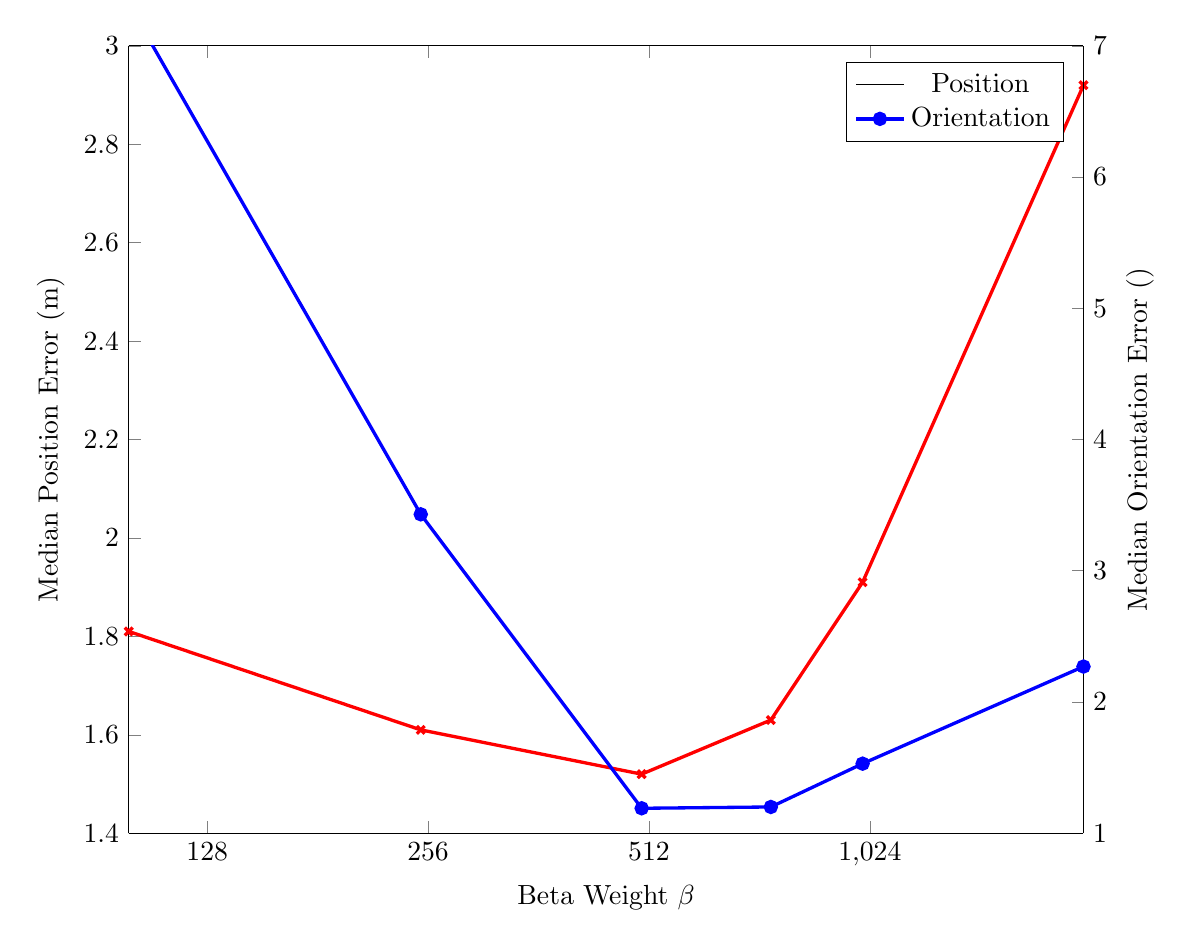
\begin{tikzpicture}
\pgfplotsset{
    compat=1.3,
    scale only axis,
    height=10cm,
    width=\columnwidth %-\widthof{100}-0.1cm, % \textwidth minus width of longest label text minus label offset
    %legend pos =north east,
}

\begin{axis}[
  xmode=log,
  log ticks with fixed point,
  axis y line*=left,
  ymin=1.4, ymax=3.0,
  xlabel=Beta Weight $\beta$,
  ylabel=Median Position Error (m),
  xmin=100, xmax=2000,
    log basis x={2},
    xticklabel=\pgfmathparse{2^\tick}\pgfmathprintnumber{\pgfmathresult},
]
\addplot[mark=x,red,very thick]
  coordinates{
    (100,1.81)
    (250,1.61)
    (500,1.52)
    (750,1.63)
    (1000,1.91)
    (2000,2.92)
}; \label{plot_one1}
\addlegendentry{Position}
\end{axis}

\begin{axis}[
  xmode=log,
  log ticks with fixed point,
  axis y line*=right,
  xtick=\empty,
  ymin=1.0, ymax=7.0,
  ylabel=Median Orientation Error ($\degree$),
  xmin=100, xmax=2000,
]
\addlegendimage{/pgfplots/refstyle=plot_one1}\addlegendentry{Position}
\addplot[mark=*,blue,very thick]
  coordinates{
    (100,7.32)
    (250,3.43)
    (500,1.19)
    (750,1.20)
    (1000,1.53)
    (2000,2.27)
};
\addlegendentry{Orientation}
\end{axis}
\end{tikzpicture}}
 
	\caption[Model performance against a range of scale factors.]{Relative performance of position and orientation regression on \textbf{a single model with a range of scale factors} for an indoor scene from the King's College scene in Cambridge Landmarks, using the loss function in \eqn{loss1}. This demonstrates that learning with the optimum scale factor leads to the network uncovering a more accurate pose function.}
\label{fig:scalefactor}
\end{figure}

\subsubsection{Learning an Optimal Weighting}
\label{sec:learn_loss}

Ideally, we would like a loss function which is able to learn position and orientation optimally, without including any hyper parameters. For this reason, we use the multi-task loss function from \cref{sec:mlttask}, which is able to learn a weighting between the position and orientation objective functions. We formulate it using \textit{homoscedastic uncertainty} which we can learn using probabilistic deep learning \citep{kendall2017uncertainties}. Homoscedastic uncertainty is a measure of uncertainty which does not depend on the input data, as opposed to heteroscedastic uncertainty which is a function of the input data \citep{kendall2017uncertainties}. Rather, it captures the uncertainty of the task itself. In \citep{kendall2017multi} we show how to use this insight to combine losses for different tasks in a probabilistic manner. Here we show how to apply this to learn camera position and orientation (with a Gaussian likelihood):
\begin{equation}
\label{eqn:loss4}
\mathcal{L}_{\sigma}(I) = \mathcal{L}_x(I) \hat{\sigma}_x^{-2} + \log{\hat{\sigma}_x^2} + \mathcal{L}_{q}(I) \hat{\sigma}_q^{-2} + \log{\hat{\sigma}_q^2}
\end{equation}
where we optimise the homoscedastic uncertainties, $\hat{\sigma}_x^2$, $\hat{\sigma}_q^2$, through backpropagation with respect to the loss function. These uncertainties are free scalar values, not model outputs. They represent the homoscedastic (task) noise.

This loss consists of two components; the residual regressions and the uncertainty regularization terms. We learn the variance, $\sigma^2$, implicitly from the loss function. As the variance is larger, it has a tempering effect on the residual regression term; larger variances (or uncertainty) results in a smaller residual loss. The second regularization term prevents the network from predicting infinite uncertainty (and therefore zero loss). As we expect quaternion values to have much smaller values (they are constrained to the unit manifold), their noise, $\sigma_q^2$ should be much smaller than the position noise, $\sigma_x^2$, which can be many meters in magnitude. As $\sigma_q^2$ should be much smaller than $\sigma_x^2$, orientation regression should be weighted much higher than position -- with a similar effect to $\beta$ in \eqn{loss1}.

In practice, we learn $\hat{s}:=\log\hat{\sigma}^2$ because it is more numerically stable \citep{kendall2017multi}:
\begin{equation}
\label{eqn:loss5}
\mathcal{L}_{\sigma}(I) = \mathcal{L}_x(I) \exp (-\hat{s}_x) + \hat{s}_x + \mathcal{L}_{q}(I) \exp (-\hat{s}_q) + \hat{s}_q
\end{equation}
This is more numerically stable than regressing the variance, $\sigma^2$, because the loss avoids a potential division by zero. The exponential mapping also allows us to regress unconstrained scalar values, where $\exp(-s_i)$ is resolved to the positive domain giving valid values for variance. We find that this loss is very robust to our initialisation choice for the homoscedastic task uncertainty values. Only an approximate initial guess is required, we arbitrarily use initial values of $\hat{s}_x=0.0, \hat{s}_q=-3.0$, for all scenes.

\subsubsection{Learning from Geometric Reprojection Error}
\label{sec:reproj}

Perhaps a more desirable loss is one that does not require balancing of rotational and positional quantities at all. Reprojection error of scene geometry is a representation which combines rotation and translation naturally in a single scalar loss \citep{hartley2000}. Reprojection error is given by the residual between 3-D points in the scene projected onto a 2-D image plane using the ground truth and predicted camera pose. It therefore converts rotation and translation quantities into image coordinates. This naturally weights translation and rotation quantities depending on the scene and camera geometry.

To formulate this loss, we first define a function, $\uppi$, which maps a 3-D point, $\mathbf{g}$, to 2-D image coordinates, $(u,v)^T$:
\begin{equation}
\uppi (\mathbf{x},\mathbf{q},\mathbf{g}) \mapsto \begin{pmatrix} u \\ v \end{pmatrix}
\end{equation}
where $\mathbf{x}$ and $\mathbf{q}$ represent the camera position and orientation. This function, $\uppi$, is defined as:
\begin{equation}
\begin{pmatrix} u' \\ v' \\ w' \end{pmatrix} = \mathsf{K} ( \mathsf{R} \mathbf{g} + \mathbf{x}), 
~~\begin{pmatrix} u \\ v \end{pmatrix} = \begin{pmatrix} u'/w' \\ v'/w' \end{pmatrix}
\end{equation}
where $\mathsf{K}$ is the intrinsic calibration matrix of the camera, and $\mathsf{R}$ is the mapping of $\mathbf{q}$ to its $SO(3)$ rotation matrix, $\textbf{q}_{4\times1} \mapsto \mathsf{R}_{3\times3}$.

We formulate this loss by taking the norm of the reprojection error between the predicted and ground truth camera pose. We take the subset, $\mathcal{G'}$, of all 3-D points in the scene, $\mathcal{G}$, which are visible in the image $I$. The final loss \eqn{loss_reproject} is given by the mean of all the residuals from points, $g_i \in \mathcal{G'}$:
\begin{equation}
\mathcal{L}_g(I) = \dfrac{1}{|\mathcal{G}'|} \sum\limits_{g_i \in \mathcal{G}'} \left\lVert \uppi (\mathbf{x},\mathbf{q},\mathbf{g_i}) - \uppi (\mathbf{\hat{x}},\mathbf{\hat{q}},\mathbf{g_i}) \right\rVert_\gamma
\label{eqn:loss_reproject}
\end{equation}
where $\mathbf{\hat{x}}$ and $\mathbf{\hat{q}}$ are the predicted camera poses from PoseNet, with $\mathbf{x}$ and $\mathbf{q}$ the ground truth label, with norm, $\gamma$, which is discussed in \sct{norm}.

Note that because we are projecting 3-D points using both the ground truth and predicted camera pose we can apply any arbitrary camera model, as long as we use the same intrinsic parameters for both cameras. Therefore for simplicity, we set the camera intrinsics, $K$, to the identity matrix -- camera calibration is not required.

This loss implicitly combines rotation and translational quantities into image coordinates. Minimising reprojection error is often the most desirable balance between these quantities for many applications, such as augmented reality. The key advantage of this loss is that it allows the model to vary the weighting between position and orientation, depending on the specific geometry in the training image. For example, training images with geometry which is far away would balance rotational and translational loss differently to images with geometry very close to the camera.

Interestingly, when experimenting with the original weighted loss in \eqn{loss1} we observed that the hyperparameter $\beta$ was an approximate function of the scene geometry. We observed that it was a function of the landmark distance and size in the scene. Our intuition was that the optimal choice for $\beta$ was approximating the reprojection error in the scene geometry. For example, if the scene is very far away, then rotation is more significant than translation and vice versa. This function is not trivial to model for complex scenes with a large number of landmarks. It will vary significantly with each training example in the dataset. By learning with reprojection error we can use our knowledge of the scene geometry more directly to automatically infer this weighting.

Projecting geometry through a projection model is a differentiable operation involving matrix multiplication. Therefore we can use this loss to train our model with stochastic gradient descent. It is important to note that we do not need to know the intrinsic camera parameters to project this 3-D geometry. This is because we apply the same projection to both the model prediction and ground truth measurement, so we can use arbitrary values.

It should be noted that we need to have some knowledge of the scene's geometry in order to have 3-D points to reproject. The geometry is often known; if our data is obtained through structure from motion, RGBD data or other sensory data (see \sct{data}). Only points from the scene which are visible in the image $I$ are used to compute the loss. We also found it was important for numerical stability to ignore points which are projected outside the image bounds.

\begin{table}[t]
	\centering
\begin{subtable}{\linewidth} \centering
	\begin{tabular}{l|ccc}
& \multicolumn{2}{c}{Median Error} & Accuracy \\
Loss function & x [$m$] & q [$\degree$] & $<2m, 5\degree$ [$\%$] \\ \hline \hline
 Linear sum, $\beta=500$ \eqn{loss1} & 1.52 & 1.19 & 65.0\% \\
 Learn weighting with homoscedastic uncertainty \eqn{loss4} & 0.99 & 1.06 & 85.3\% \\ \hline
 Reprojection loss & \multicolumn{3}{c}{does not converge} \\ \hline
 Learn weighting pretraining $\mapsto$ Reprojection loss \eqn{loss_reproject} & 0.88 & 1.04 & 90.3\% \\
	\end{tabular}
    \caption{Cambridge Landmarks, King's College}
\end{subtable}

\begin{subtable}{\linewidth} \centering
	\begin{tabular}{l|ccc}
& \multicolumn{2}{c}{Median Error} & Accuracy \\
Loss function & x [$m$] & q [$\degree$] & $<2m, 5\degree$ [$\%$] \\ \hline \hline
 Linear sum, $\beta=500$ \eqn{loss1} & 13.1 & 4.68 & 30.1\% \\
 Learn weighting with homoscedastic uncertainty \eqn{loss4} & 9.88 & 4.73 & 41.7\% \\ \hline
 Reprojection loss & \multicolumn{3}{c}{does not converge} \\ \hline
 Learn weighting pretraining $\mapsto$ Reprojection loss \eqn{loss_reproject} & 7.90 & 4.40 & 48.6\% \\
	\end{tabular}
    \caption{Dubrovnik 6K}
\end{subtable}
	\caption[Effect of varying loss functions on localisation performance.]{\textbf{Comparison of different loss functions.} We use an $L_1$ distance for the residuals in each loss. \textit{Linear sum} combines position and orientation losses with a constant scaling parameter $\beta$ \citep{kendall2015modelling} and is defined in \eqn{loss1}. Learn weighting is the loss function in \eqn{loss4} which learns to combine position and orientation using homoscedastic uncertainty. Reprojection error implicitly combines rotation and translation by using the reprojection error of the scene geometry as the loss \eqn{loss_reproject}. We find that homoscedastic uncertainty is able to learn an effective weighting between position and orientation quantities. The reprojection loss was not able to converge from random initialisation. However, when used to fine-tune a network pretrained with \eqn{loss4} it yields the best results.}
	\label{tbl:losses}
\end{table}

\subsubsection{Regression Norm}
\label{sec:norm}

An important choice for these losses is the regression norm, $\left\lVert~\right\rVert_\gamma$. Typically, deep learning models use an $L_1 = \left\lVert~\right\rVert_1$ or $L_2 = \left\lVert~\right\rVert_2$. We can also use robust norms such as Huber's loss \citep{huber2011robust} and Tukey's loss \citep{hoaglin1983understanding}, which have been successfully applied to deep learning \citep{belagiannis2015robust}. For camera pose regression, we found that they negatively impacted performance by over-attenuating difficult examples. We suspect that for more noisy datasets these robust regression functions might be beneficial. With the datasets used in this chapter, we found the $L_1$ norm to perform best and therefore use use $\gamma=1$. It does not increase quadratically with magnitude or over-attenuate large residuals.

\section{Localisation Experiments}
\label{sec:exp}

To train and benchmark our model on a number of datasets we rescale the input images such that the shortest side is of length 256. We normalise the images so that input pixel intensities range from $-1$ to $1$. We train our PoseNet architecture using an implementation in TensorFlow \citep{abadi2016tensorflow}. All models are optimised end-to-end with ADAM \citep{kingma2014adam} using the default parameters and a learning rate of $1 \times 10^{-4}$. We train each model until the training loss converges. We use a batch size of 64 on a NVIDIA Titan X (Pascal) GPU, training takes approximately 20k - 100k iterations, or 4 hours - 1 day.

\subsection{Datasets}
\label{sec:data}

\begin{figure}[p]
\centering

	\begin{subfigure}[t]{\linewidth}
	\resizebox{\linewidth}{!}{
		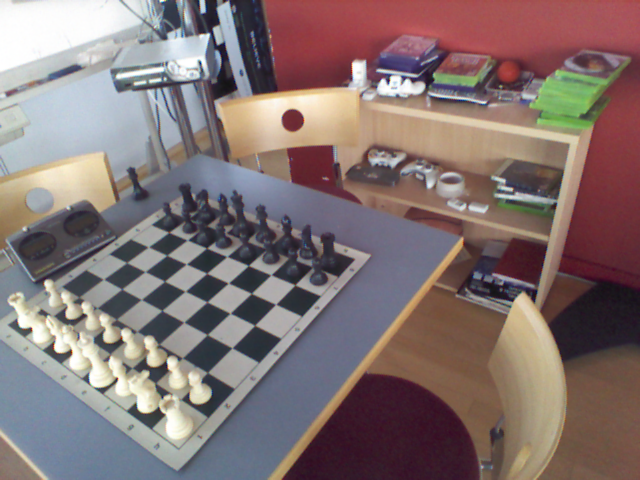
\includegraphics[width=0.2\linewidth]{Datasets/chess.png}
		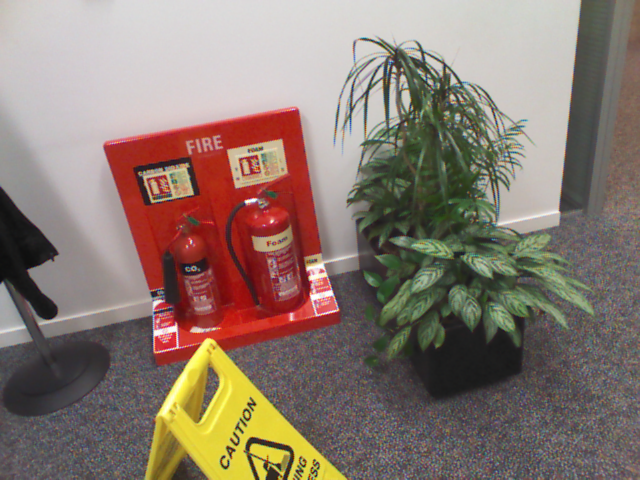
\includegraphics[width=0.2\linewidth]{Datasets/fire.png}
		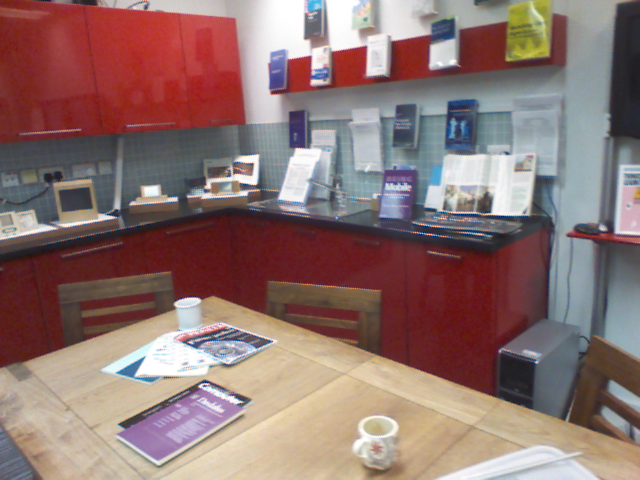
\includegraphics[width=0.2\linewidth]{Datasets/kitchen.png}
		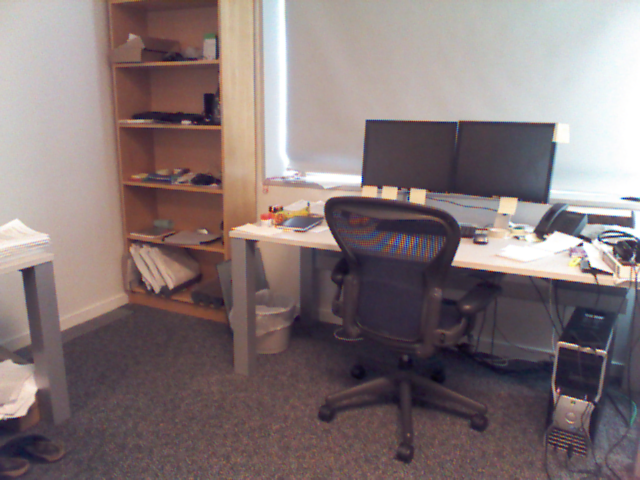
\includegraphics[width=0.2\linewidth]{Datasets/office.png}
		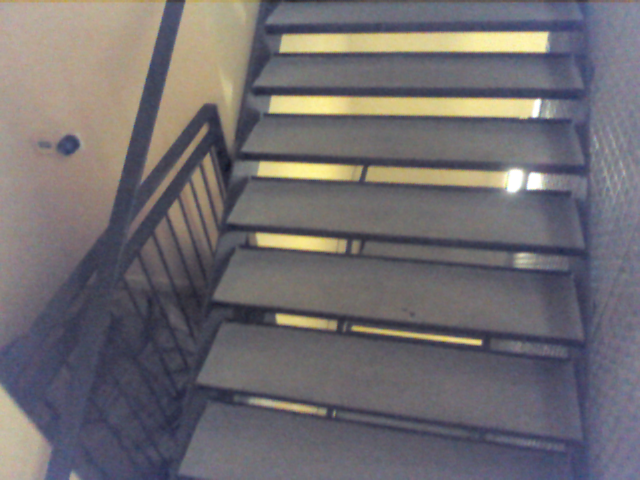
\includegraphics[width=0.2\linewidth]{Datasets/stairs.png}
		}
	\caption{7 Scenes Dataset - 43,000 images from seven scenes in small indoor environments \citep{shotton2013scene}.}
	~
	~
	\end{subfigure}
	
	\begin{subfigure}[t]{\linewidth}
	\resizebox{\linewidth}{!}{
		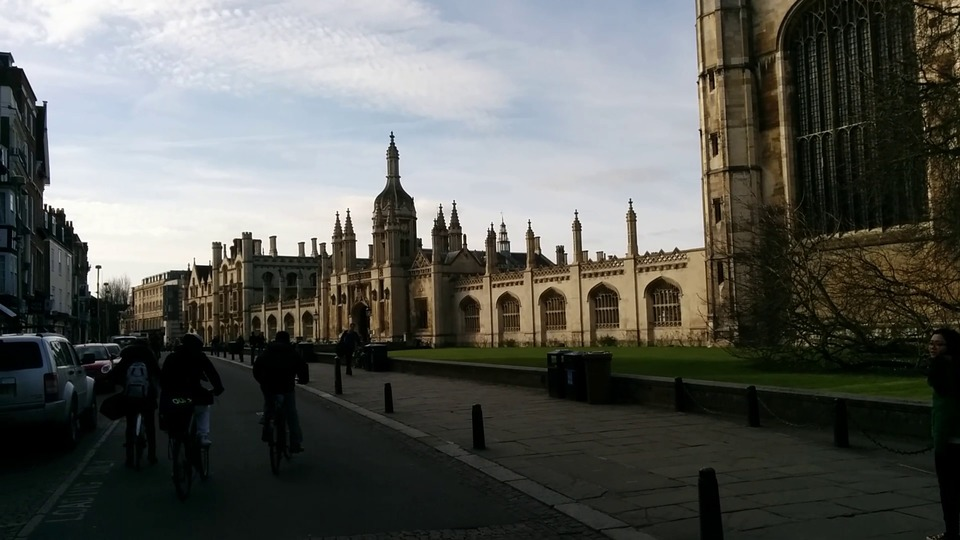
\includegraphics[width=0.2\linewidth]{Datasets/frame00015.jpg}
		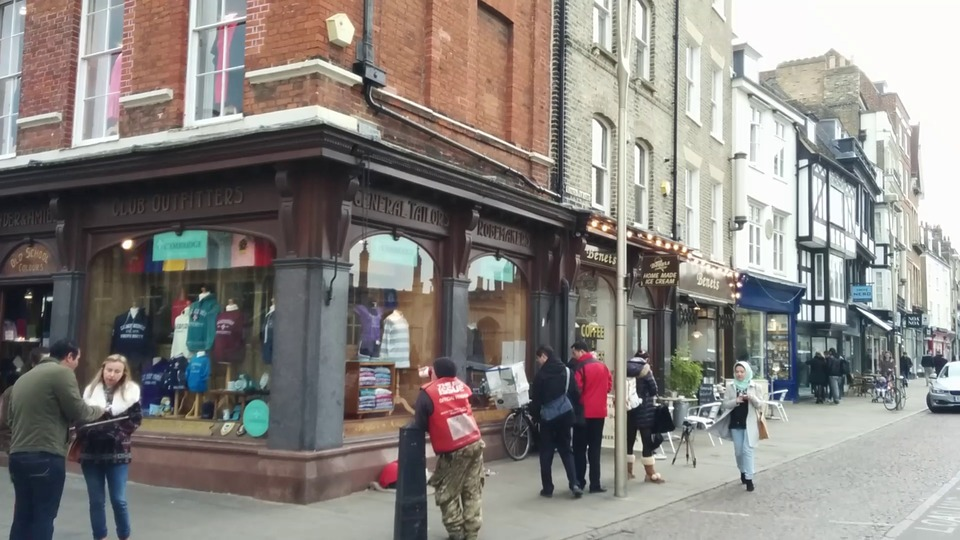
\includegraphics[width=0.2\linewidth]{Datasets/frame00016.jpg}
		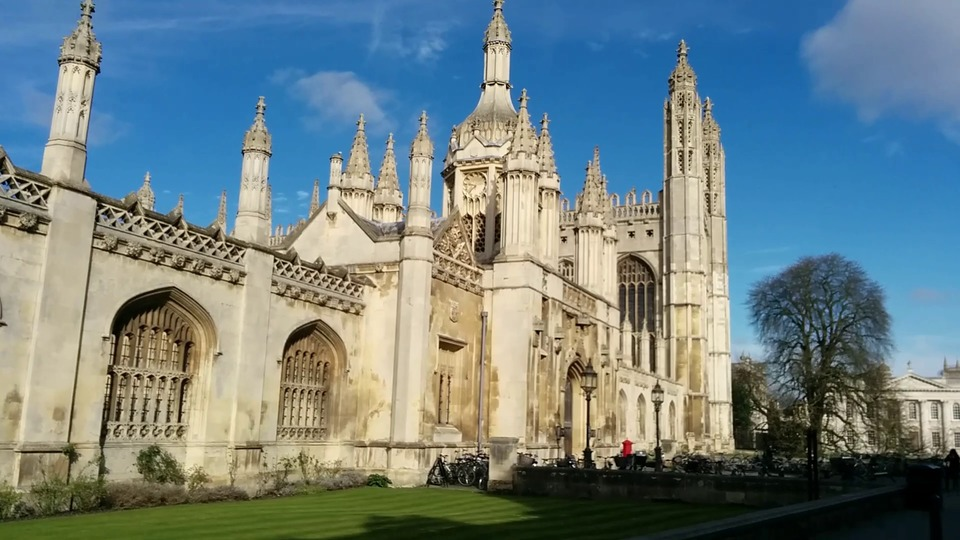
\includegraphics[width=0.2\linewidth]{Datasets/frame00428.jpg}
		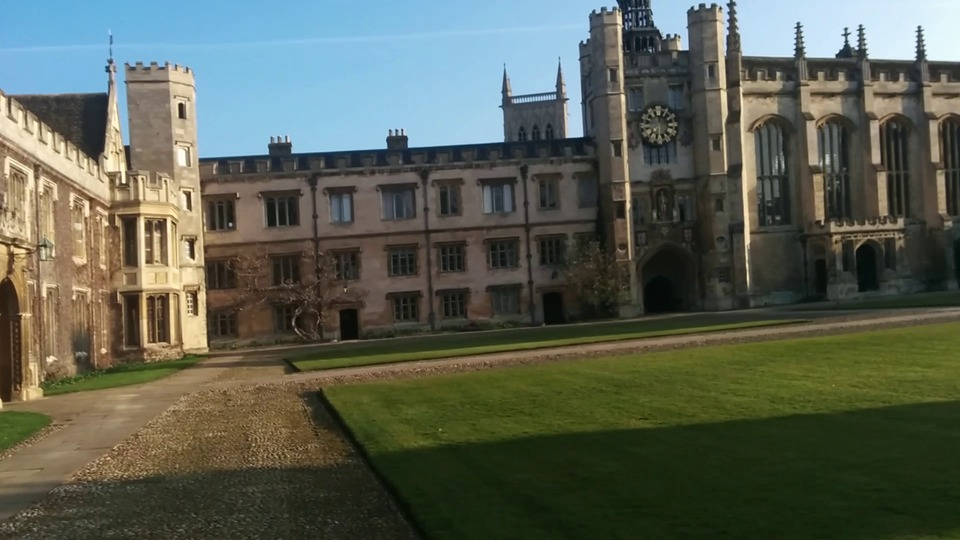
\includegraphics[width=0.2\linewidth]{Datasets/frame00599.jpg}
		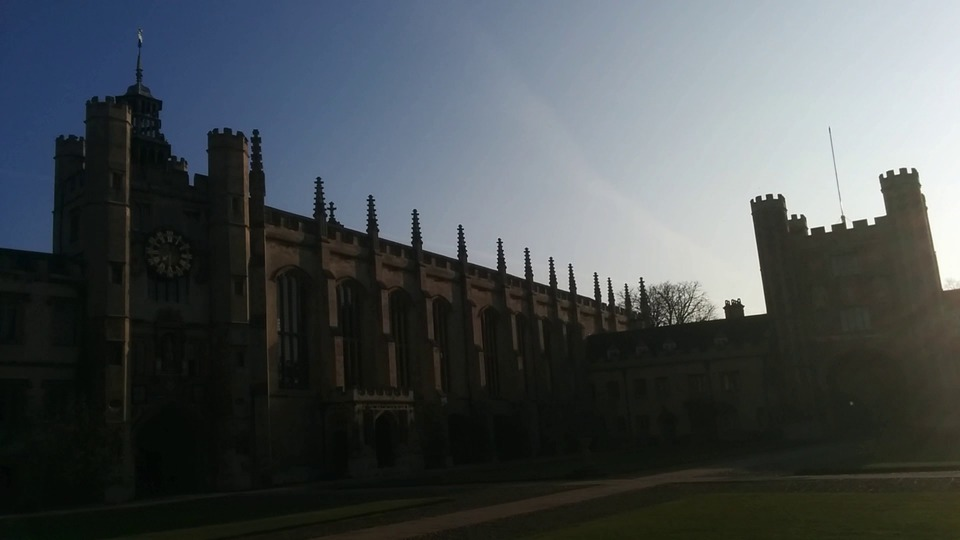
\includegraphics[width=0.2\linewidth]{Datasets/frame00615.jpg}
		}
        
    \vspace{0.5mm}
	\resizebox{\linewidth}{!}{
		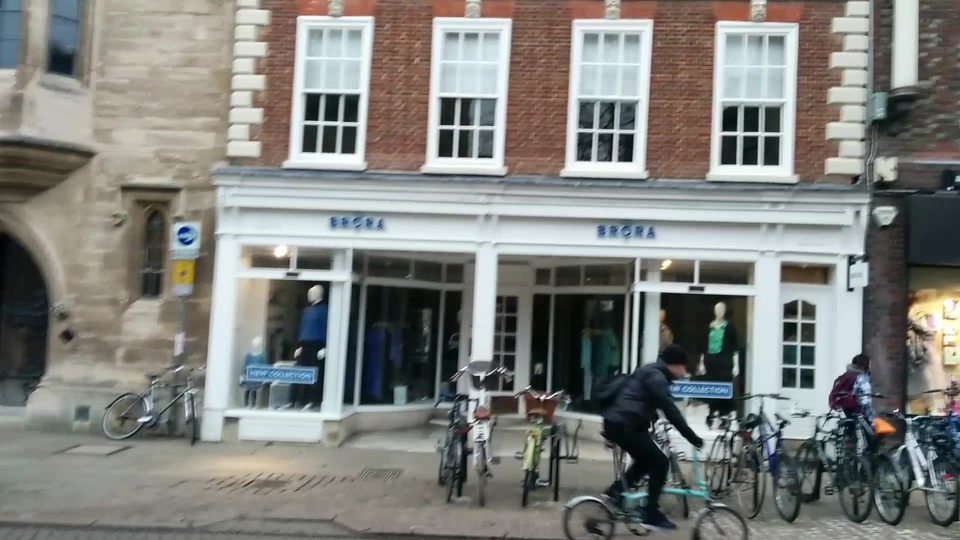
\includegraphics[width=0.2\linewidth]{Datasets/image1_000031.jpg}
		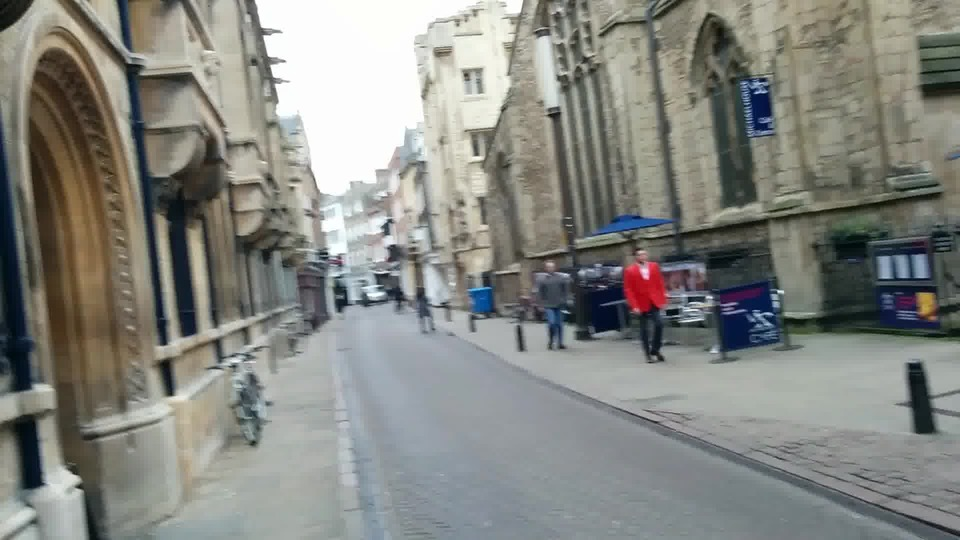
\includegraphics[width=0.2\linewidth]{Datasets/image2_000585.jpg}
		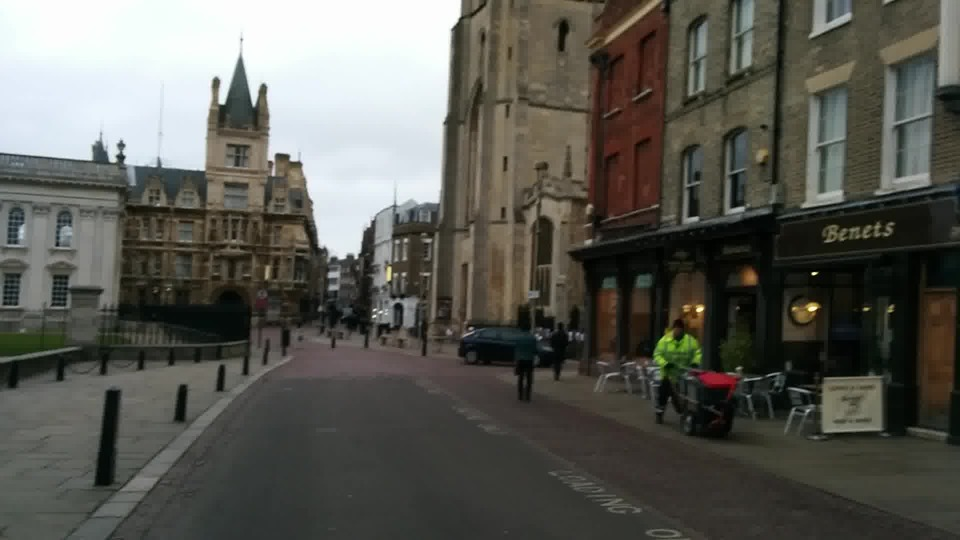
\includegraphics[width=0.2\linewidth]{Datasets/image2_001336.jpg}
		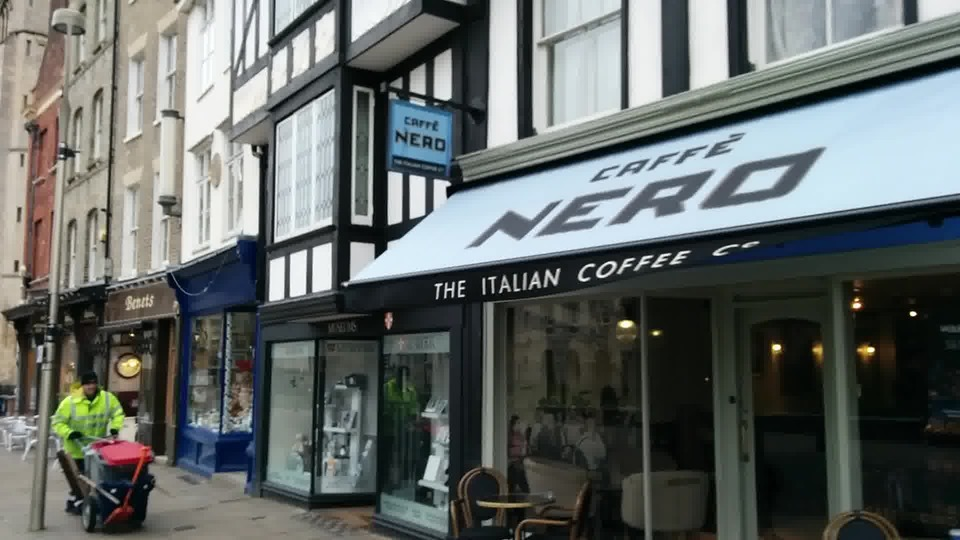
\includegraphics[width=0.2\linewidth]{Datasets/image2_001351.jpg}
		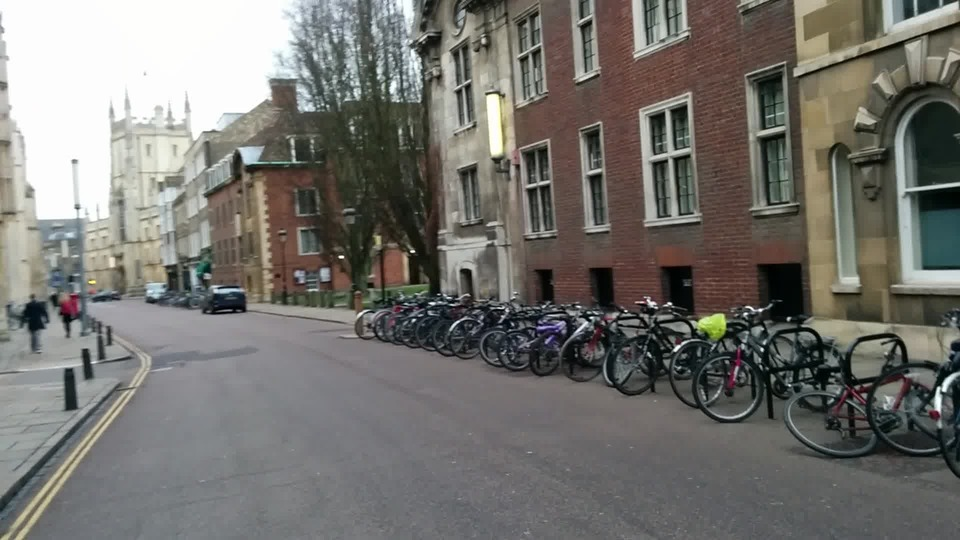
\includegraphics[width=0.2\linewidth]{Datasets/image2_002421.jpg}
		}
	\caption{Cambridge Landmarks Dataset - over 10,000 images from six scenes around Cambridge, UK \citep{kendall2015posenet}.}
	~
	~
	\end{subfigure}
	
	\begin{subfigure}[t]{\linewidth}
	\resizebox{\linewidth}{!}{
		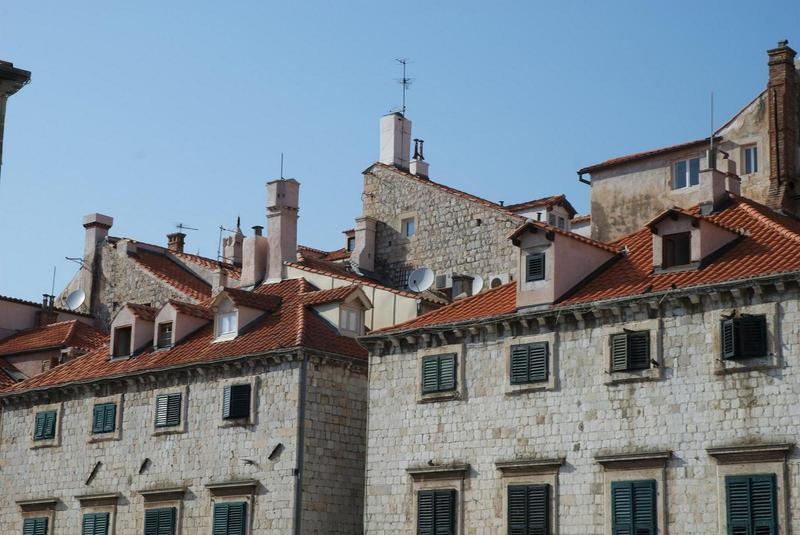
\includegraphics[height=50mm]{Datasets/5n4k3_2760651317.jpg}
		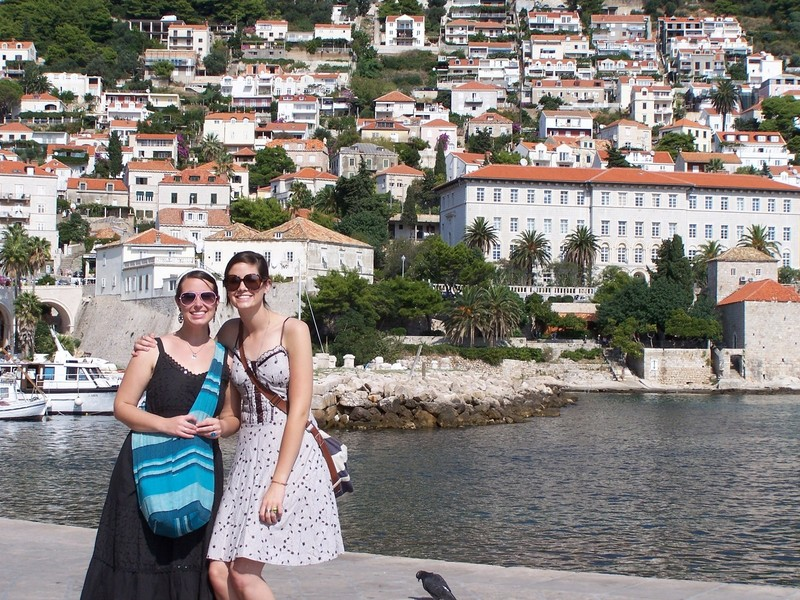
\includegraphics[height=50mm]{Datasets/5pointloperist_2921626253.jpg}
		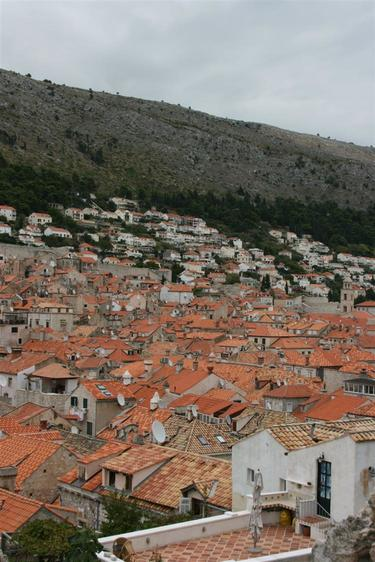
\includegraphics[height=50mm]{Datasets/709913_2965924825.jpg}
		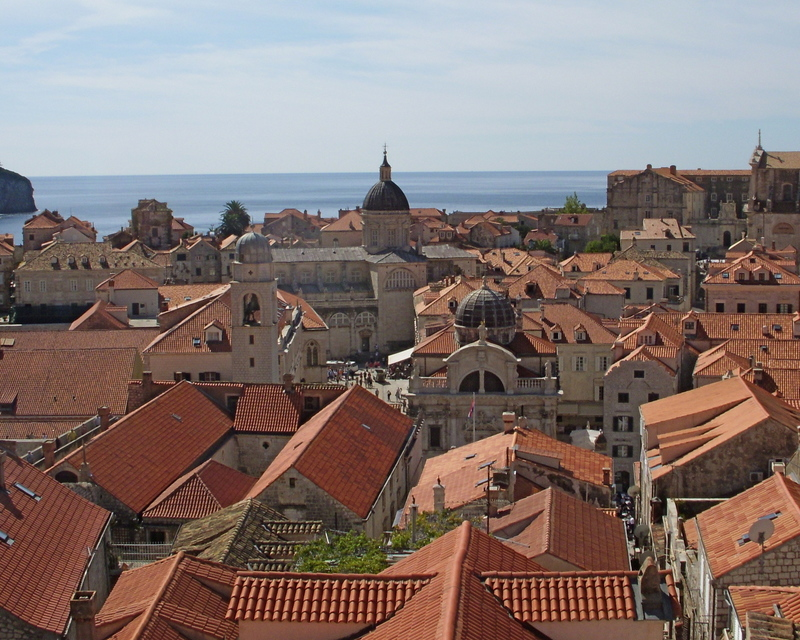
\includegraphics[height=50mm]{Datasets/7145465_N07_3065208814.jpg}
		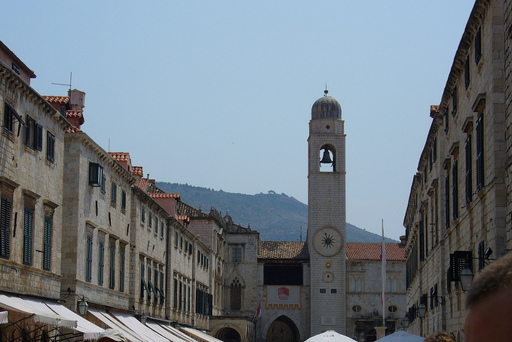
\includegraphics[height=50mm]{Datasets/7286581_N04_2243494109.jpg}
		}
        
    \vspace{0.5mm}
	\resizebox{\linewidth}{!}{
		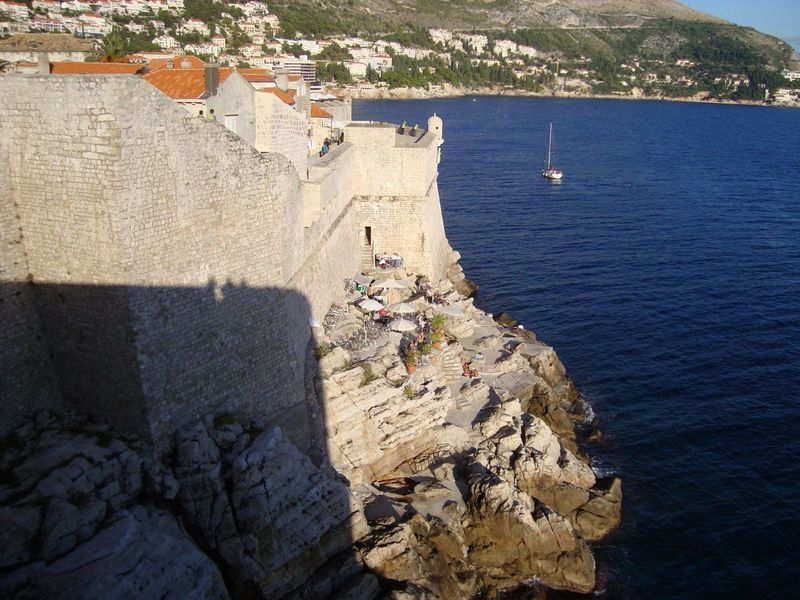
\includegraphics[height=50mm]{Datasets/8117903_N06_2955594865.jpg}
		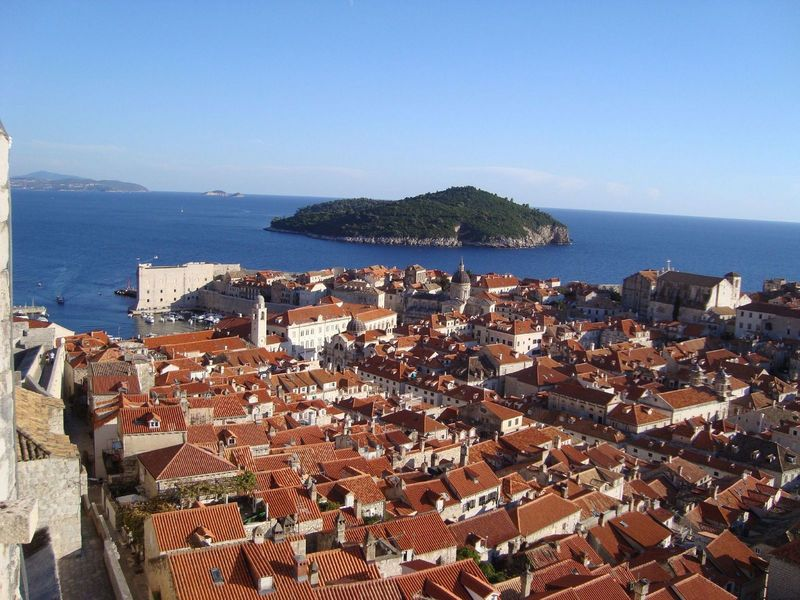
\includegraphics[height=50mm]{Datasets/8117903_N06_2956436946.jpg}
		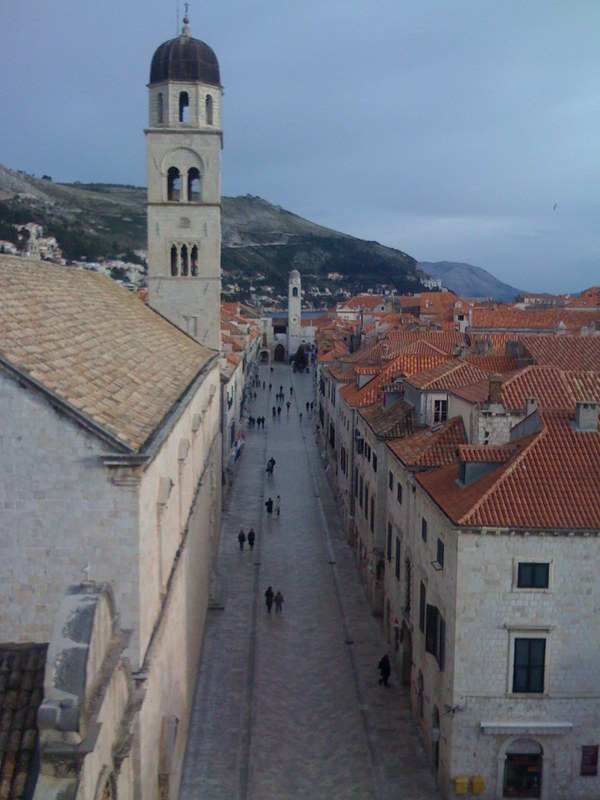
\includegraphics[height=50mm]{Datasets/8223442_N02_3167519460.jpg}
		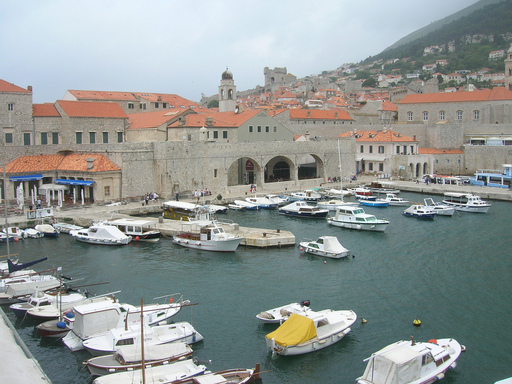
\includegraphics[height=50mm]{Datasets/10970812_N05_2553025324.jpg}
		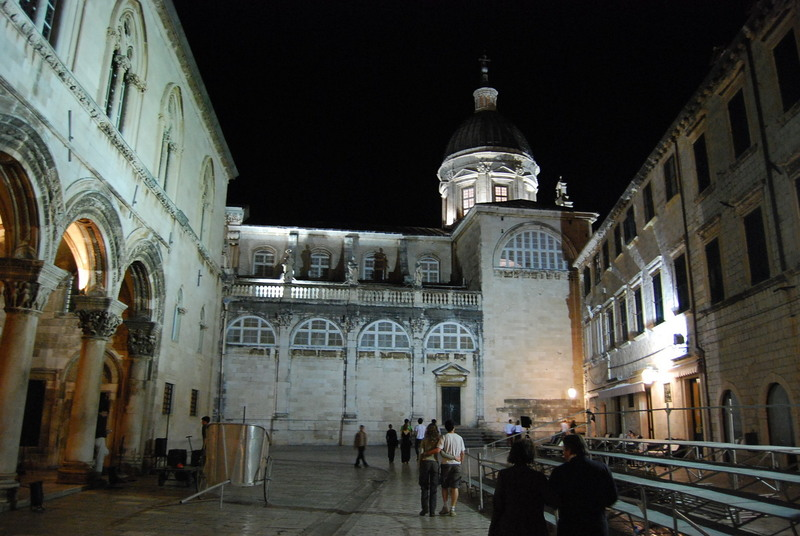
\includegraphics[height=50mm]{Datasets/16798538_N06_1808716980.jpg}
		}
	\caption{Dubrovnik 6K Dataset - 6,000 images from a variety of camera types in Dubrovnik, Croatia \citep{li2010location}.}
	~
	~
	\end{subfigure}
	
\caption[Localisation datasets.]{\textbf{Example images randomly chosen from each dataset.} This illustrates the wide variety of settings and scales and the challenging array of environmental factors such as lighting, occlusion, dynamic objects and weather which are captured in each dataset.}
\label{fig:datasets}
\end{figure}


\afterpage{%
    \clearpage% Flush earlier floats (otherwise order might not be correct)
    \begin{landscape}% Landscape page
    \centering
\begin{table*}[t]
	\centering
	\resizebox{\linewidth}{!}{
	\begin{tabular}{l|c|c|c|c|c|c|c|c}
		Dataset & Type & Scale & Imagery & Scenes & Train Images & Test Images & 3-D Points & Spatial Area \\ \hline \hline
		7 Scenes & Indoor & Room & RGB-D sensor (Kinect) & 7 & 26,000 & 17,000 & - & 4$\times$3m \\
		Cambridge Landmarks & Outdoor & Street & Mobile phone camera & 6 & 8,380 & 4,841 & 2,097,191 & 100$\times$500m \\
		Dubrovnik 6K & Outdoor & Small town & Internet images (Flikr) & 1 & 6,044 & 800 & 2,106,456 & 1.5$\times$1.5km \\
		%San Francisco (SF1) & Outdoor & Large city & Vehicle camera & 1 & 790,000 & 800 & 75,410,077 & 4$\times$4km\\
	\end{tabular}}
	\caption[Localisation dataset details.]{\textbf{Summary of the localisation datasets used in this chapter's experiments.} We compare 7 Scenes \citep{shotton2013scene}, Cambridge Landmarks \citep{kendall2015posenet}, Dubrovnik \citep{li2012worldwide} and the San Francisco \citep{chen2011city} datasets. These datasets are all publicly available. They demonstrate our method's performance over a range of scales for both indoor and outdoor applications.}
	\label{tbl:datasets}
\end{table*}
\end{landscape}
\clearpage% Flush page
}

Deep learning performs extremely well on large datasets. However annotating ground truth labels on these datasets is often expensive or very labour intensive. We can leverage structure from motion \citep{Snavely08IJCV}, or similar algorithms \citep{shotton2013scene}, to autonomously generate training labels (camera poses) from image data \citep{kendall2015posenet}. We use three datasets to benchmark our approach. These datasets are summarised in \tbl{datasets} and example imagery is shown in \fig{datasets}. We use these datasets to demonstrate our method's performance across a range of settings and scales. We endeavour to demonstrate the general applicability of the approach.

\textbf{Cambridge Landmarks} \citep{kendall2015posenet} provides labelled video data to train and test pose regression algorithms in an outdoor urban setting. It was collected using a smart phone and structure from motion was used to generate the pose labels \citep{wu2013towards}. Significant urban clutter such as pedestrians and vehicles were present and data was collected from many different points in time representing different lighting and weather conditions. Train and test images are taken from distinct walking paths and not sampled from the same trajectory making the regression challenging.

\textbf{7 Scenes} \citep{shotton2013scene} is an indoor dataset which was collected with a Kinect RGB-D sensor. Ground truth poses were computed using Kinect Fusion \citep{shotton2013scene}. The dataset contains seven scenes which were captured around an office building. Each scene typically consists of a single room. The dataset was originally created for RGB-D relocalisation. It is extremely challenging for purely visual relocalisation using SIFT-like features, as it contains many ambiguous textureless features.

\textbf{Dubrovnik 6K} \citep{li2012worldwide} is a dataset consisting of 6,044 train and 800 test images which were obtained from the internet. They are taken from Dubrovnik's old town in Croatia which is a UNESCO world heritage site. The images are predominantly captured by tourists with a wide variety of camera types. Ground truth poses for this dataset were computed using structure from motion.

\subsection{Comparison of Loss Functions}
\label{sec:loss_exp}

In \tbl{losses} we compare different combinations of losses and regression norms. We compare results for a scene in the Cambridge Landmarks dataset \citep{kendall2015posenet} and the Dubrovnik 6K dataset \citep{li2012worldwide}, which has imagery from a range of cameras.

We find that modelling homoscedastic uncertainty with the loss in \eqn{loss4} is able to effectively learn a weighting between position and orientation. It outperforms the constant weighting used in loss \eqn{loss1}. The reprojection loss in \eqn{loss_reproject} is unable to train the model from a random initialisation. We observe that the model gets stuck in a poor local minima, when using any of the regression norms. However, the reprojection loss is able to improve localisation performance when using weights pretrained with any of the other losses. For example, we can take the best performing model using the loss from \eqn{loss4} and fine tune with the reprojection loss \eqn{loss_reproject}. We observe that this loss is then able to converge effectively. This shows that the reprojection loss is not robust to large residuals. This is because reprojected points can be easily placed far from the image centre if the network makes a poor pose prediction. Therefore, we recommend the following two-step training scheme:
\begin{enumerate}
  \item Train the model using the loss in \eqn{loss4}, learning the weighting between position and orientation.
  \item If the scene geometry is known (for example from structure from motion or RGBD camera data) then fine-tune the model using the reprojection loss in \eqn{loss_reproject}.
\end{enumerate}

\afterpage{%
    \clearpage% Flush earlier floats (otherwise order might not be correct)
    \begin{landscape}% Landscape page
    \centering
\begin{table*}[t]
\begin{center}
	\resizebox{\linewidth}{!}{
\begin{tabular}{l|c|c c c c c c}
 & Area or & Active Search (SIFT) & PoseNet ($\beta$ weight) & Bayesian PoseNet & PoseNet Spatial LSTM & PoseNet & PoseNet\\
Scene & Volume & \citep{sattler2016efficient} & \citep{kendall2015posenet} & \citep{kendall2015modelling} &  \citep{walch2016image} & Learn $\sigma^2$ Weight & Geometric Reprojection\\
\hline \hline
Great Court	 		& $8000m^2$		& -- 				 &	--				  &	--			   	   & -- 				& 7.00m, 3.65\degree & 6.83m, 3.47\degree \\
King's College 		& $5600m^2$ 	& 0.42m, 0.55\degree & 1.66m, 4.86\degree & 1.74m, 4.06\degree & 0.99m, 3.65\degree & 0.99m, 1.06\degree & 0.88m, 1.04\degree \\
Old Hospital 		& $2000m^2$ 	& 0.44m, 1.01\degree & 2.62m, 4.90\degree & 2.57m, 5.14\degree & 1.51m, 4.29\degree & 2.17m, 2.94\degree & 3.20m, 3.29\degree \\
Shop Fa\c cade 		& $875m^2$ 		& 0.12m, 0.40\degree & 1.41m, 7.18\degree & 1.25m, 7.54\degree & 1.18m, 7.44\degree & 1.05m, 3.97\degree & 0.88m, 3.78\degree \\
St Mary's Church 	& $4800m^2$ 	& 0.19m, 0.54\degree & 2.45m, 7.96\degree & 2.11m, 8.38\degree & 1.52m, 6.68\degree & 1.49m, 3.43\degree & 1.57m, 3.32\degree \\
Street 				& $50000m^2$ 	& 0.85m, 0.83\degree & -- 				  & -- 				   & --					& 20.7m, 25.7\degree & 20.3m, 25.5\degree \\
\hline
\multicolumn{5}{c}{}\\
\hline
Chess 		& $6m^3$ 	& 0.04m, 1.96\degree & 0.32m, 6.60\degree & 0.37m, 7.24\degree & 0.24m, 5.77\degree & 0.14m, 4.50\degree & 0.13m, 4.48\degree \\
Fire 		& $2.5m^3$ 	& 0.03m, 1.53\degree & 0.47m, 14.0\degree & 0.43m, 13.7\degree & 0.34m, 11.9\degree & 0.27m, 11.8\degree & 0.27m, 11.3\degree \\
Heads 		& $1m^3$ 	& 0.02m, 1.45\degree & 0.30m, 12.2\degree & 0.31m, 12.0\degree & 0.21m, 13.7\degree & 0.18m, 12.1\degree & 0.17m, 13.0\degree \\
Office 		& $7.5m^3$ 	& 0.09m, 3.61\degree & 0.48m, 7.24\degree & 0.48m, 8.04\degree & 0.30m, 8.08\degree & 0.20m, 5.77\degree & 0.19m, 5.55\degree \\
Pumpkin 	& $5m^3$ 	& 0.08m, 3.10\degree & 0.49m, 8.12\degree & 0.61m, 7.08\degree & 0.33m, 7.00\degree & 0.25m, 4.82\degree & 0.26m, 4.75\degree \\
Red Kitchen & $18m^3$	& 0.07m, 3.37\degree & 0.58m, 8.34\degree & 0.58m, 7.54\degree & 0.37m, 8.83\degree & 0.24m, 5.52\degree & 0.23m, 5.35\degree \\
Stairs 		& $7.5m^3$ 	& 0.03m, 2.22\degree & 0.48m, 13.1\degree & 0.48m, 13.1\degree & 0.40m, 13.7\degree & 0.37m, 10.6\degree & 0.35m, 12.4\degree \\
\hline
\end{tabular}}
\end{center}

	\caption[Localisation results for Cambridge Landmarks and 7 Scenes.]{\textbf{Median localisation results for the \textit{Cambridge Landmarks} \citep{kendall2015posenet} and \textit{7 Scenes} \citep{shotton2013scene} datasets.} We compare the performance of various RGB-only algorithms. Active search \citep{sattler2016efficient} is a state-of-the-art traditional SIFT keypoint based baseline. We demonstrate a notable improvement over PoseNet's \citep{kendall2015posenet} baseline performance using the learned $\sigma^2$ and reprojection error proposed in this chapter, narrowing the margin to the state of the art SIFT technique.}
	\label{tbl:mainresults}
\end{table*}
\end{landscape}
\clearpage% Flush page
}

\subsection{Benchmarking Localisation Accuracy}
\label{sec:benchmark}

In \tbl{mainresults} we show that our geometry based loss outperforms the original PoseNet's naive loss function \citep{kendall2015posenet}. We observe a consistent and significant improvement across both indoor \textit{7 Scenes} outdoor \textit{Cambridge Landmarks} datasets. We conclude that we can simultaneously learn both position and orientation more effectively by considering scene geometry. The improvement is notably more pronounced for the 7Scenes dataset. We believe this is due to the significantly larger amount of training data for each scene in this dataset, compared with Cambridge Landmarks. We also outperform the improved PoseNet architecture with spatial LSTMs \citep{walch2016image}. However, this method is complimentary to the loss functions in this chapter, and it would be interesting to explore the union of these ideas.

We observe a difference in relative performance between position and orientation when optimising with respect to reprojection error \eqn{loss_reproject} or homoscedastic uncertainty \eqn{loss4}. Overall, optimising reprojection loss improves rotation accuracy, sometimes at the expense of some positional precision.

\subsection{Comparison to SIFT-Feature Approaches}

\tbl{mainresults} also compares to a state-of-the-art traditional SIFT feature based localisation algorithm, Active Search \citep{sattler2016efficient}. This method outperforms PoseNet, and is effective in feature-rich outdoor environments. However, in the 7Scenes dataset this deficit is less pronounced. The indoor scenes contain much fewer point features and there is significantly more training data. As an explanation for the deficit in these results, PoseNet only uses $256\times 256$ pixel images, while SIFT based methods require images of a few mega-pixels in size \citep{sattler2016efficient}. Additionally, PoseNet is able to localise an image in $5ms$, scaling constantly with scene area, while traditional SIFT feature approaches require over $100ms$, and scale with scene size \citep{sattler2016efficient}.

In \tbl{dubrovnik_results} we compare our approach on the Dubrovnik dataset to other geometric techniques which localise by registering SIFT features \citep{lowe2004distinctive} to a large 3-D model \citep{li2012worldwide}. Although our method improves significantly over the original PoseNet model, it is still yet to reach the fine grained accuracy of these methods \citep{svarm2014accurate,zeisl2015camera,sattler2011fast,li2010location}. We hypothesise that this is due to a lack of training data, with only 6k images across the town. However, our algorithm is significantly faster than these approaches. Furthermore, it is worth noting that PoseNet only sees a $256\times256$ resolution image, while these methods register the full size images, often with a few million pixels.
	
\begin{table}[t]
	\centering
	\begin{tabular}{l|cc|cc}
		& \multicolumn{2}{c|}{Position} & \multicolumn{2}{c}{Orientation} \\
		Method & Mean [m] & Median [m] & Mean [$\degree$] & Median [$\degree$] \\ \hline \hline
		PoseNet (this work) & 40.0 & 7.9 & 11.2 & 4.4 \\
		APE \citep{svarm2014accurate} & - & 0.56 & - & - \\
		Voting \citep{zeisl2015camera} & - & 1.69 & - & - \\
		Sattler, et al. \citep{sattler2011fast} & 14.9 & 1.3 & - & - \\
		P2F \citep{li2010location} & 18.3 & 9.3 & - & - \\
	\end{tabular}
	\caption[Localisation results for the Dubrovnik dataset.]{\textbf{Localisation results on the Dubrovnik dataset} \citep{li2012worldwide}, comparing to a number of state-of-the-art point-feature techniques. Our method is the first deep learning approach to benchmark on this challenging dataset. We achieve comparable performance, while our method only requires a 256$\times$256 pixel image and is much faster to compute.}
	\label{tbl:dubrovnik_results}
\end{table}




\begin{figure}[t]
   	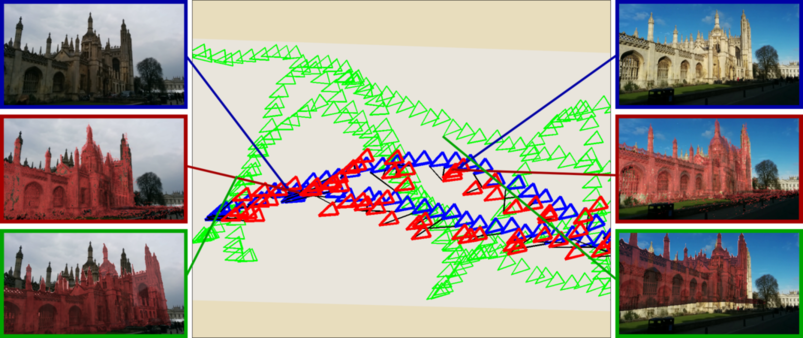
\includegraphics[width=\linewidth]{ICCV/zoominmap}
   \caption[Localisation results over train and test sequences.]{Magnified view of a sequence of \textbf{training (green)} and \textbf{testing (blue)} cameras for King's College. We show the \textbf{predicted camera pose in red} for each testing frame. The images show the test image (top), the predicted view from our model overlaid in red on the input image (middle) and the nearest neighbour training image overlaid in red on the input image (bottom). This shows our system can interpolate camera pose effectively in space between training frames.}
\label{fig:zoommap}
\end{figure}

\begin{figure}[t]
\makebox[\textwidth][c]{
   	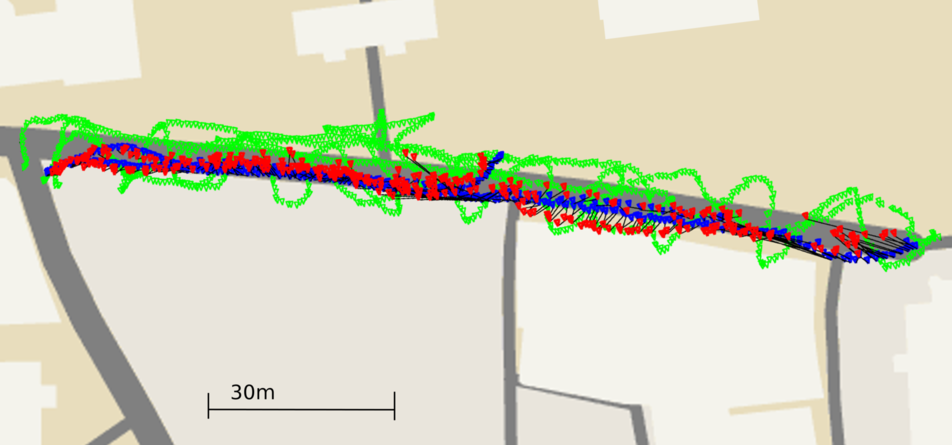
\includegraphics[height=0.2\linewidth]{ICCV/kingsmap}
   	~
   	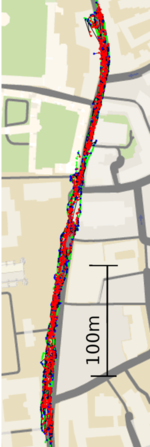
\includegraphics[height=0.2\linewidth]{ICCV/kpmap}
   	~
   	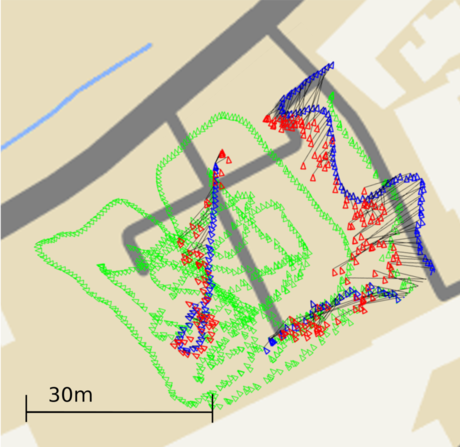
\includegraphics[height=0.2\linewidth]{ICCV/jbsmap}
   	~
   	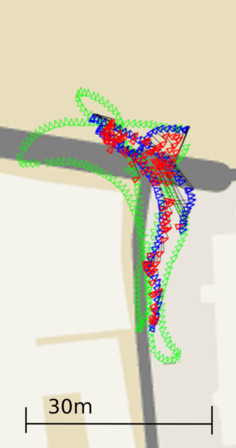
\includegraphics[height=0.2\linewidth]{ICCV/ramap}
   	~
   	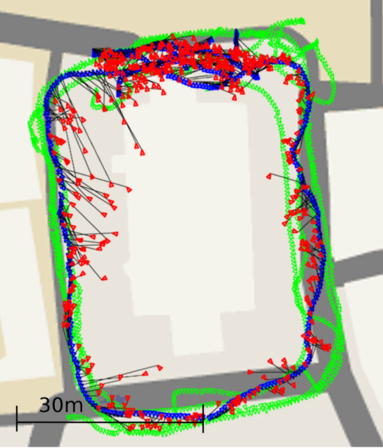
\includegraphics[height=0.2\linewidth]{ICCV/stmarysmap}
   	}
\makebox[\textwidth][l]{
\makebox[0.44\textwidth][c]{
\textit{King's College}
   	}
\makebox[0.03\textwidth][c]{
\textit{Street}
   	}
\makebox[0.24\textwidth][c]{
\textit{Old Hospital}
   	}
\makebox[0.1\textwidth][c]{
\textit{Shop Fa\c cade}
   	}
\makebox[0.2\textwidth][c]{
\textit{St Mary's Church}
   	}}
   \caption[Map of Cambridge Landmarks dataset.]{\textbf{Map of dataset} showing training frames (green), testing frames (blue) and their predicted camera pose (red). The testing sequences are distinct trajectories from the training sequences and each scene covers a very large spatial extent.}
   \label{fig:map}
\end{figure}






\begin{figure}[p]
\clearpage% Flush page
\begin{center}
\vspace{-7mm}
\begin{subfigure}[b]{\textwidth}
\makebox[\textwidth][c]{
   	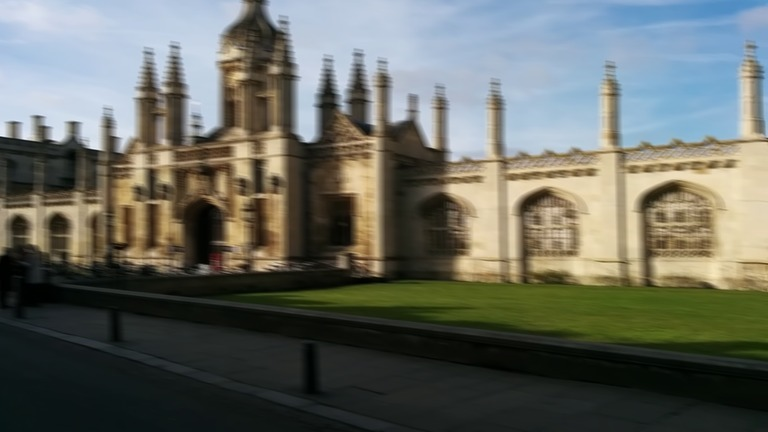
\includegraphics[width=0.16\linewidth]{ICCV/kings_seq3_frame00110_blur25}
   	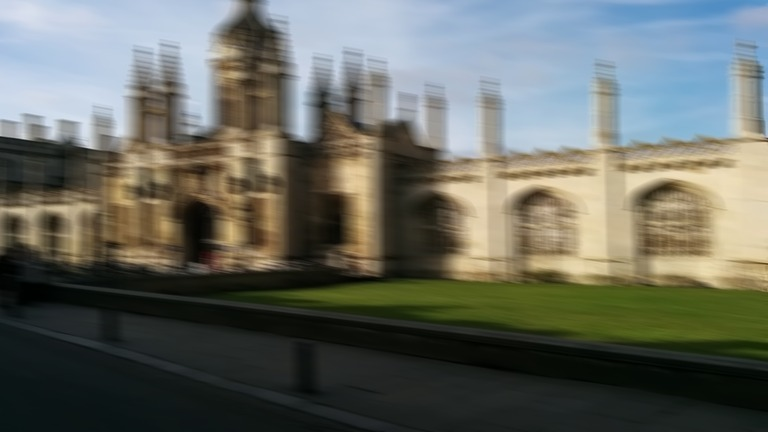
\includegraphics[width=0.16\linewidth]{ICCV/kings_seq3_frame00110_blur50}
   	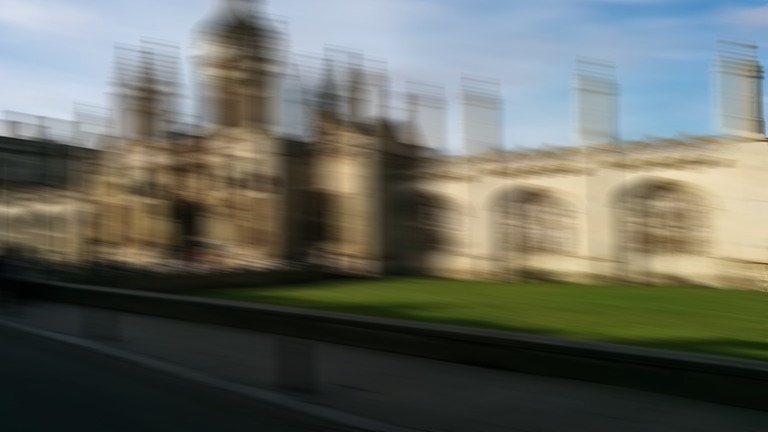
\includegraphics[width=0.16\linewidth]{ICCV/kings_seq3_frame00110_blur100}
   	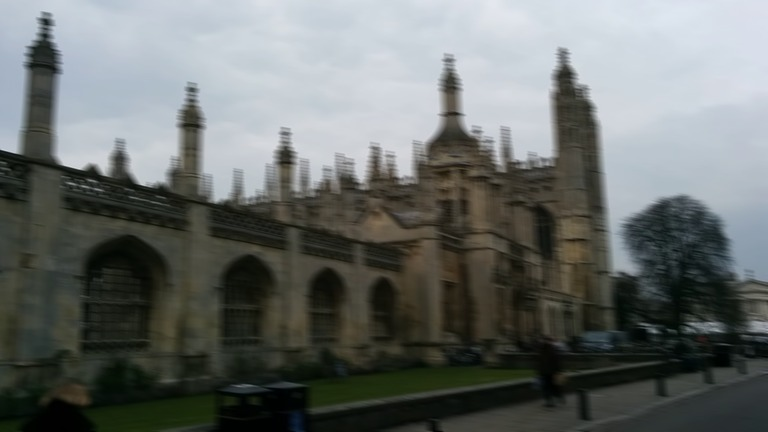
\includegraphics[width=0.16\linewidth]{ICCV/kings_seq7_frame00010_blur25}
   	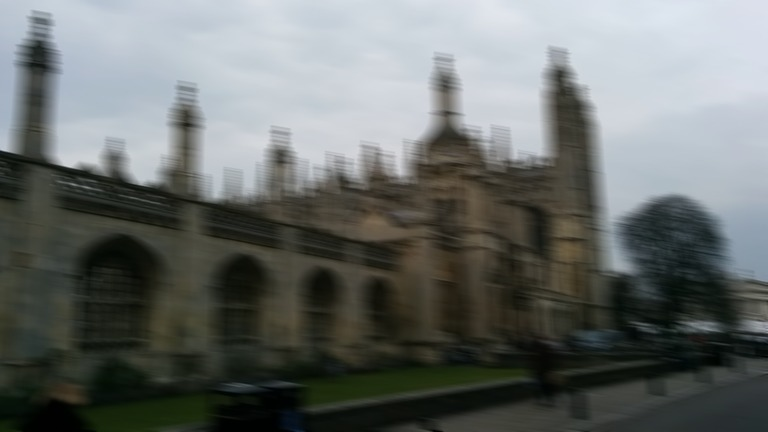
\includegraphics[width=0.16\linewidth]{ICCV/kings_seq7_frame00010_blur50}
   	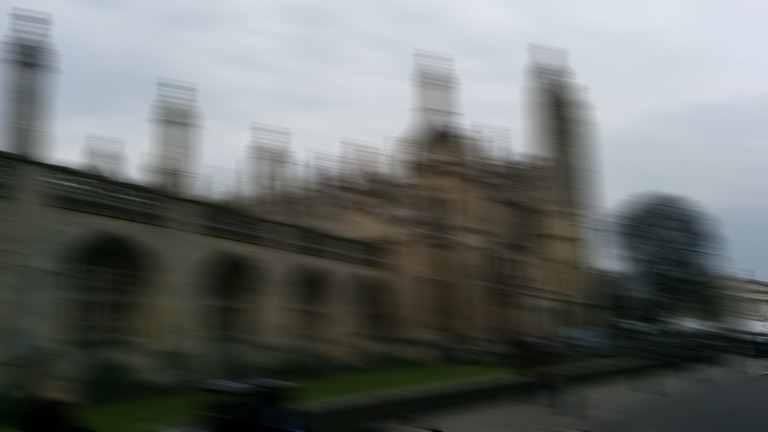
\includegraphics[width=0.16\linewidth]{ICCV/kings_seq7_frame00010_blur100}
   	}
\makebox[\textwidth][c]{
   	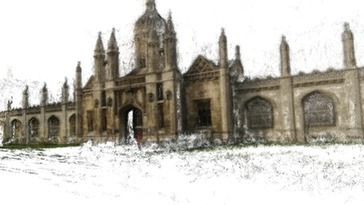
\includegraphics[width=0.16\linewidth]{ICCV/king_seq3_frame00110_blur25pngscreenshot}
   	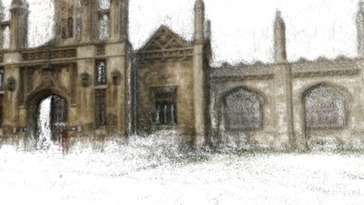
\includegraphics[width=0.16\linewidth]{ICCV/king_seq3_frame00110_blur50pngscreenshot}
   	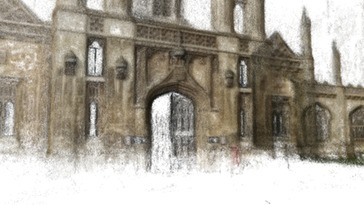
\includegraphics[width=0.16\linewidth]{ICCV/king_seq3_frame00110_blur100pngscreenshot}
   	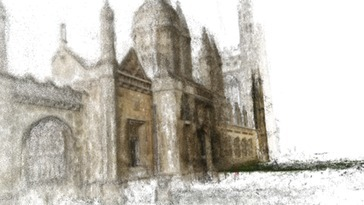
\includegraphics[width=0.16\linewidth]{ICCV/king_seq7_frame00010_blur25pngscreenshot}
   	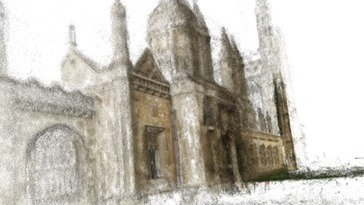
\includegraphics[width=0.16\linewidth]{ICCV/king_seq7_frame00010_blur50pngscreenshot}
   	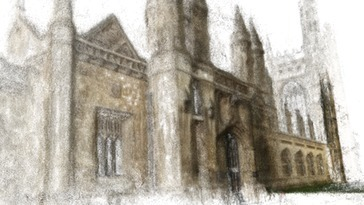
\includegraphics[width=0.16\linewidth]{ICCV/king_seq7_frame00010_blur100pngscreenshot}
   	}
   \caption{Relocalisation with increasing levels of motion blur. The system is able to recognize the pose as high level features such as the contour outline still exist. Blurring the landmark increases apparent contour size and the system believes it is closer. }
\end{subfigure}

\begin{subfigure}[b]{\textwidth}
\makebox[\textwidth][c]{
   	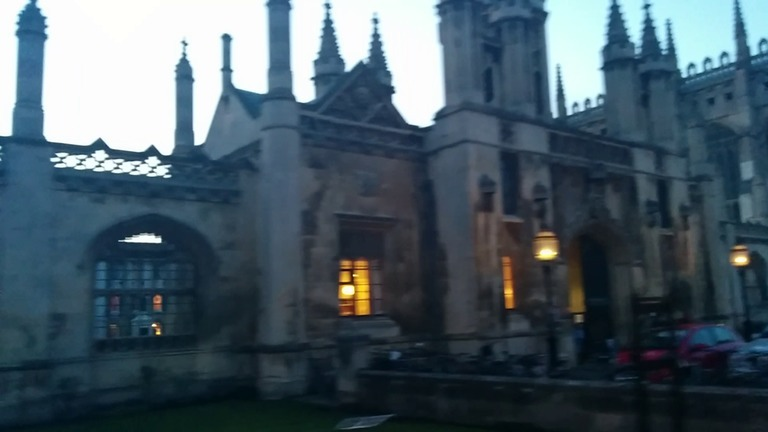
\includegraphics[width=0.24\linewidth]{ICCV/frame00023}
   	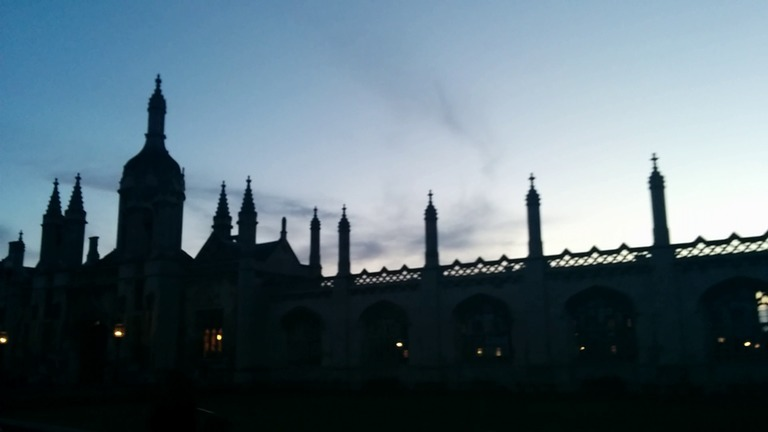
\includegraphics[width=0.24\linewidth]{ICCV/frame00048}
   	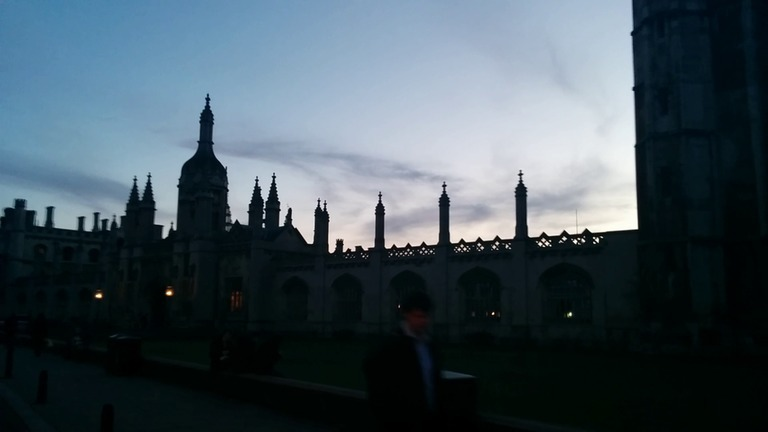
\includegraphics[width=0.24\linewidth]{ICCV/frame00054}
   	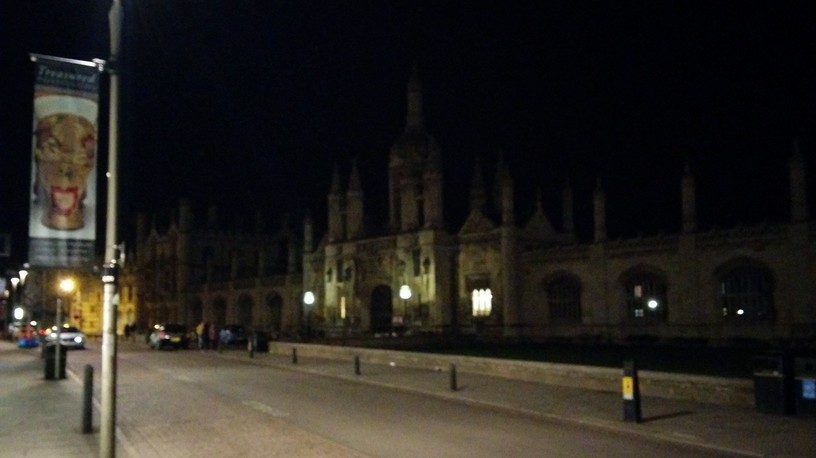
\includegraphics[width=0.24\linewidth]{ICCV/IMG_20150418_230453}
   	}
\makebox[\textwidth][c]{
   	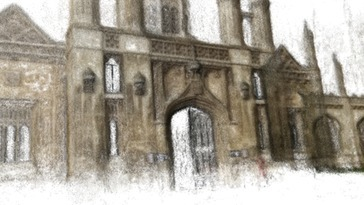
\includegraphics[width=0.24\linewidth]{ICCV/fram00023pngscreenshot}
   	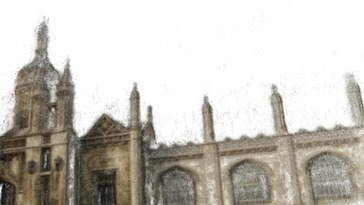
\includegraphics[width=0.24\linewidth]{ICCV/fram00048pngscreenshot}
   	\includegraphics[width=0.24\linewidth]{ICCV/fram00054pngscreenshot}
   	\includegraphics[width=0.24\linewidth]{ICCV/IMG_20150418_230453jpgscreenshot}
   	}
\makebox[\textwidth][c]{
   	\includegraphics[width=0.24\linewidth]{ICCV/fram00023pngoverlay}
   	\includegraphics[width=0.24\linewidth]{ICCV/fram00048pngoverlay}
   	\includegraphics[width=0.24\linewidth]{ICCV/fram00054pngoverlay}
   	\includegraphics[width=0.24\linewidth]{ICCV/IMG_20150418_230453jpgoverlay}
   	}
   \caption{Relocalisation under difficult dusk and night lighting conditions. In the dusk sequences, the landmark is silhouetted against the backdrop however again the model seems to recognize the contours and estimate pose.}
\end{subfigure}

\vspace{-5mm}
\begin{subfigure}[t]{0.28\textwidth}
\makebox[\textwidth][c]{
   	\includegraphics[width=0.5\textwidth]{ICCV/frame00029}
   	\includegraphics[width=0.5\textwidth]{ICCV/frame00060}
   	}
\makebox[\textwidth][c]{
   	\includegraphics[width=0.5\textwidth]{ICCV/fram00029pngscreenshot}
   	\includegraphics[width=0.5\textwidth]{ICCV/fram00060pngscreenshot}
   	}
\makebox[\textwidth][c]{
   	\includegraphics[width=0.5\textwidth]{ICCV/fram00029pngoverlay}
   	\includegraphics[width=0.5\textwidth]{ICCV/fram00060pngoverlay}
   	}
   \caption{Relocalisation with different weather conditions. PoseNet is able to effectively estimate pose in fog and rain.}
\end{subfigure}
\qquad
\begin{subfigure}[t]{0.28\textwidth}
\makebox[\textwidth][c]{
   	\includegraphics[width=0.5\textwidth]{ICCV/frame00037}
   	\includegraphics[width=0.5\textwidth]{ICCV/frame00008}
   	}
\makebox[\textwidth][c]{
   	\includegraphics[width=0.5\textwidth]{ICCV/seq2frame00037pngscreenshot}
   	\includegraphics[width=0.5\textwidth]{ICCV/seq1frame00008pngscreenshot}
   	}
\makebox[\textwidth][c]{
   	\includegraphics[width=0.5\textwidth]{ICCV/seq2frame00037pngoverlay}
   	\includegraphics[width=0.5\textwidth]{ICCV/seq1frame00008pngoverlay}
   	}
   \caption{Relocalisation with significant people, vehicles and other dynamic objects.}
\end{subfigure}
\qquad
\begin{subfigure}[t]{0.28\textwidth}
\makebox[\textwidth][c]{
   	\includegraphics[width=0.5\textwidth]{ICCV/img1}
   	\includegraphics[width=0.5\textwidth]{ICCV/frame00051}
   	}
\makebox[\textwidth][c]{
   	\includegraphics[width=0.5\textwidth]{ICCV/img1jpgscreenshot}
   	\includegraphics[width=0.5\textwidth]{ICCV/seq2frame00051pngscreenshot}
   	}
\makebox[\textwidth][c]{
   	\includegraphics[width=0.5\textwidth]{ICCV/img1jpgoverlay}
   	\includegraphics[width=0.5\textwidth]{ICCV/seq2frame00051pngoverlay}
   	}
   \caption{Relocalisation with unknown camera intrinsics: SLR with focal length 45mm (left), and iPhone 4S with focal length 35mm (right) compared to the dataset's camera which had a focal length of 30mm.}
\end{subfigure}
\end{center}
\vspace{-5mm}
	\caption[Robustness to challenging real life situations.]{\textbf{Robustness to challenging real life situations.} Registration with point based techniques such as SIFT fails in examples (a-c), therefore ground truth measurements are not available. None of these types of challenges were seen during training. As convolutional neural networks are able to understand objects and contours they are still successful at estimating pose from the building's contour in the silhouetted examples (b) or even under extreme motion blur (a). Many of these quasi invariances were enhanced by pretraining from the scenes dataset.}
	\label{fig:difficultexamples}
\clearpage% Flush page
\end{figure}

We show that PoseNet is able to effectively localize across both the indoor \textit{7 Scenes} dataset and outdoor \textit{Cambridge Landmarks} dataset in \cref{tbl:mainresults}. To validate that the model is regressing pose beyond that of the training examples we show the performance for finding the nearest neighbour representation in the training data from the feature vector produced by the localisation network. As our performance exceeds this we conclude that the network is successfully able to regress pose beyond training examples (see \cref{fig:zoommap}). We also compare our algorithm to the RGB-D SCoRe Forest algorithm \citep{shotton2013scene}. 

\begin{figure*}[t]
\makebox[\textwidth][c]{
   	\includegraphics[width=0.26\linewidth]{ICCV/kings}
   	\includegraphics[width=0.26\linewidth]{ICCV/businessschool}
   	\includegraphics[width=0.26\linewidth]{ICCV/pumpkin}
   	\includegraphics[width=0.26\linewidth]{ICCV/stairs}
   	}
   \caption[Localisation histograms.]{\textbf{Localization performance.} These figures show our localization accuracy for both position and orientation as a cumulative histogram of errors for the entire training set. The regression network outperforms the nearest neighbour feature matching which demonstrates we regress finer resolution results than given by training. Comparing to the RGB-D SCoRe Forest approach shows that our method is competitive, but outperformed by a more expensive depth approach. Our method does perform better on the hardest few frames, above the 95th percentile, with our worst error lower than the worst error from the SCoRe approach. }
   \label{fig:histograms}
\end{figure*}

\cref{fig:histograms} shows cumulative histograms of localisation error for two indoor and two outdoor scenes. We note that although the SCoRe forest is generally more accurate, it requires depth information, and uses higher-resolution imagery. The indoor dataset contains many ambiguous and textureless features which make relocalisation without this depth modality extremely difficult. We note our method often localizes the most difficult testing frames, above the 95th percentile, more accurately than SCoRe across all the scenes. We also observe that dense cropping only gives a modest improvement in performance. It is most important in scenes with significant clutter like pedestrians and cars, for example King's College, Shop Fa\c cade and St Mary's Church.

We explored the robustness of this method beyond what was tested in the dataset with additional images from dusk, rain, fog, night and with motion blur and different cameras with unknown intrinsics. \cref{fig:difficultexamples} shows the convolutional neural network generally handles these challenges well. SfM with SIFT fails in all these cases so we were not able to generate a ground truth camera pose, however we infer the accuracy by viewing the 3-D reconstruction from the predicted camera pose, and overlaying this onto the input image.

\subsection{Robustness Against Training Image Spacing}

We demonstrate in \cref{fig:baseline} that, for an outdoor scale scene, we gain little by spacing the training images more closely than 4m. The system is robust to very large spatial separation between training images, achieving reasonable performance even with only a few dozen training samples. The pose accuracy deteriorates gracefully with increased training image spacing, whereas SIFT-based SfM sharply fails after a certain threshold as it requires a small baseline \citep{lowe2004distinctive}.

\begin{figure}[t]
\begin{center}
   	\includegraphics[width=0.7\linewidth]{ICCV/reduced_baseline}
\end{center}
   \caption[Robustness to a decreasing training baseline.]{\textbf{Robustness to a decreasing training baseline} for the King's College scene. Our system exhibits graceful decline in performance as fewer training samples are used.}
\label{fig:baseline}
\end{figure}

\subsection{Importance of Transfer Learning}

In general deep networks require large amounts of training data. We sidestep this problem by starting our pose training from a network pretrained on giant datasets such as \textit{ImageNet} and \textit{Places}. Similar to what has been demonstrated for classification tasks, \cref{fig:transfer} shows how transfer learning can be utilised effectively between classification and complicated regression tasks. Such `transfer learning' has been demonstrated elsewhere for training classifiers \citep{razavian2014cnn,oquab2014learning,bengio2013representation}, but here we demonstrate transfer learning from classification to the qualitatively different task of pose regression. It is not immediately obvious that a network trained to output pose-invariant classification labels would be suitable as a starting point for a pose regressor. We find, however, that this is not a problem in practice. A possible explanation is that, in order for its output to be invariant to pose, the classifier network must keep track of pose, to better factor its effects away from identity cues. This would agree with our own findings that a network trained to output position and orientation outperforms a network trained to output only position. By preserving orientation information in the intermediate representations, it is better able to factor the effects of orientation out of the final position estimation. Transfer learning gives not only a large improvement in training speed, but also end performance. 

The relevance of data is also important. In \cref{fig:transfer} the \textit{Places} and \textit{ImageNet} curves initially have the same performance. However, ultimately the \textit{Places} pretraining performs better due to being a more relevant dataset to this localisation task.

\begin{figure}[t]
\begin{center}
   	\adjustbox{trim={0} {0} {0} {0.05\height},clip}{\includegraphics[width=0.9\linewidth]{ICCV/transferlearning.pdf}}
\end{center}
   \caption[Importance of transfer learning.]{\textbf{Importance of transfer learning.} Shows how pretraining on large datasets gives an increase in both performance and training speed.}
\label{fig:transfer}
\end{figure}

\subsection{Visualising Features Relevant to Pose}

\begin{figure*}[t]
\makebox[\linewidth][c]{
   	\includegraphics[width=0.33\linewidth]{ICCV/img_com2_wpqr}
   	\includegraphics[width=0.33\linewidth]{ICCV/img_com7_xyz_kings}
   	\includegraphics[width=0.33\linewidth]{ICCV/img_com5_wpqr}
   	}
   \caption[Saliency maps.]{\textbf{Saliency maps.} This figure shows the saliency map superimposed on the input image. The saliency maps suggest that the convolutional neural network exploits not only distinctive point features (\`{a} la SIFT), but also large textureless patches, which can be as informative, if not more so, to the pose. This, combined with a tendency to disregard dynamic objects such as pedestrians, enables it to perform well under challenging circumstances. (Best viewed electronically.)}
\label{fig:saliency}
\end{figure*}

\cref{fig:saliency} shows example saliency maps produced by PoseNet. The saliency map, as used in \citep{simonyan2013deep}, is the magnitude of the gradient of the loss function with respect to the pixel intensities. This uses the sensitivity of the pose with respect to the pixels as an indicator of how important the network considers different parts of the image.

These results show that the strongest response is observed from higher-level features such as windows and spires. However a more surprising result is that PoseNet is also very sensitive to large textureless patches such as road, grass and sky. These textureless patches may be more informative than the highest responding points because the effect of a group of pixels on the pose variable is the sum of the saliency map values over that group of pixels. This evidence points to the net being able to localize off information from these textureless surfaces, something which interest-point based features such as SIFT or SURF fail to do.

The last observation is that PoseNet has an attenuated response to people and other noisy objects, effectively masking them. These objects are dynamic, and the model has identified them as not appropriate for localisation.

\subsection{Viewing the Internal Representation}

\begin{figure}[t]
\makebox[\linewidth][c]{
   	\framebox[\width]{ \includegraphics[width=0.35\linewidth]{ICCV/tsne_places_googlenet_on_kings_seq3}}
   	\framebox[\width]{ \includegraphics[width=0.35\linewidth]{ICCV/tsne_kingsparade_googlenet_on_kings_seq3}}
   	\framebox[\width]{ \includegraphics[width=0.35\linewidth]{ICCV/tsne_kings_googlenet_on_kings_seq3}}
   	}
\makebox[\linewidth][c]{
\makebox[0.35\linewidth][c]{
(a)
   	}
\makebox[0.35\linewidth][c]{
(b)
   	}
\makebox[0.35\linewidth][c]{
(c)
   	}}
   \caption[Feature vector visualisation.]{\textbf{Feature vector visualisation.} t-SNE visualisation of the feature vectors from a video sequence traversing an outdoor scene (King's College) in a straight line. Colour represents time. The feature representations are generated from the model with weights trained on \textit{Places} (a), \textit{Places} then another outdoor scene, St Mary's Church (b), \textit{Places} then this outdoor scene, King's College (c). Despite (a,b) not being trained on this scene, these visualizations suggest that it is possible to compute the pose as a simple, if non-linear, function of these representations.}
\label{fig:tsne}
\end{figure}

t-SNE \citep{van2008visualizing} is an algorithm for embedding high-dimensional data in a low dimensional space, in a way that tries to preserve Euclidean distances. It is often used, as we do here, to visualize high-dimensional feature vectors in two dimensions. In \cref{fig:tsne} we apply t-SNE to the feature vectors computed from a sequence of video frames taken by a pedestrian. As these figures show, the feature vectors are a function that smoothly varies with, and is largely one-to-one with, pose. This `pose manifold' can be observed not only on networks trained on other scenes, but also networks trained on classification image sets without pose labels. This further suggests that classification networks preserve pose information up to the final layer, regardless of whether it's expressed in the output. However, the mapping from feature vector to pose becomes more complicated for networks not trained on pose data. Furthermore, as this manifold exists on scenes that the model was not trained on, the model must learn some generic representation of the relationship between landmarks, geometry and camera motion. This demonstrates that the feature vector that is produced from regression is able to generalize to other tasks in the same way as classification networks.

\subsection{System Efficiency}

\begin{figure}[t]
\makebox[\linewidth][c]{
   	%\includegraphics[width=\linewidth]{ICCV/speedmemory-eps-converted-to.pdf}
   	}
   \caption[Implementation efficiency.]{\textbf{Implementation efficiency.} Experimental speed and memory use of the regression network, nearest neighbour network feature vector baseline and SIFT relocalisation methods.}
\label{fig:speed}
\end{figure}

\cref{fig:speed} compares system performance of PoseNet on a modern desktop computer. Our network is very scalable, as it only takes $50$ MB to store the weights, and $5ms$ to compute each pose, compared to the gigabytes and minutes for metric localisation with SIFT. These values are independent of the number of training samples in the system while metric localisation scales $\mathcal{O}(n^2)$ with training data size \citep{wu2013towards}. For comparison, matching to the network's nearest neighbour is also shown. This requires storing feature vectors for each training frame, then perform a linear search to find the nearest neighbour for a given test frame.

















\section{Localisation Uncertainty}
\label{loc_unc}

In this section, we extend the PoseNet framework to a Bayesian deep learning model which is able to determine the uncertainty of localisation using the ideas from \cref{seg_unc}. Our Bayesian convolutional neural network requires no additional memory, and can relocalise in under 50ms per frame on a GPU. By leveraging this probabilistic approach, we achieve 10 - 15\% improvement on state of the art performance on \textit{Cambridge Landmarks}, a vary large urban relocalisation dataset, and \textit{7 Scenes}, a challenging indoor relocalisation dataset. Furthermore, our approach qualitatively improves the system by producing a measure of model uncertainty. We leverage this uncertainty value to estimate:
\begin{itemize}
\item metric relocalisation error for both position and orientation,
\item the confidence of modelling the data (detect if the scene is actually present in the input image).
\end{itemize}

Understanding model uncertainty is an important feature for a localisation system. A non-Bayesian system which outputs point estimates does not interpret if the model is making sensible predictions or just guessing at random. By measuring uncertainty we can understand with what confidence we can trust the prediction.

Secondly, it is easy to imagine visually similar landmarks and we need to be able to understand with what confidence can we trust the result. For example, there are many examples of buildings with visually ambiguous structures, such as window, which are tessellated along a wall.

Following \cref{scene_understanding}, we conclude that it is more important to model \textit{epistemic} uncertainty for localisation. This is because training data is often sparse. Furthermore, it is critical to detect if the input image is one from the scene which the model is trained to localise with. This is also known as \textit{loop-closure}. It requires a strong ability to detect novel input images which are outside the training data distribution. In \cref{seg_unc} we show that this is something aleatoric uncertainty cannot model, therefore in this section we focus on modelling epistemic uncertainty.

\subsection{Modelling Localisation Uncertainty}

Although many of the modern SLAM algorithms do not consider localisation uncertainty \citep{klein2007parallel,engel2014lsd,li2012worldwide}, previous probabilistic algorithms have been proposed. Bayesian approaches include extended Kalman filters and particle filter approaches such as FastSLAM \citep{thrun2005probabilistic}. However these approaches estimate uncertainty from sensor noise models, not the uncertainty of the model to represent the data. Our proposed framework does not assume any input noise but measures the model uncertainty for localisation.

Neural networks which consider uncertainty are known as Bayesian neural networks \citep{denker1991transforming,mackay1992practical}. They offer a probabilistic interpretation of deep learning models by inferring distributions over the networks’ weights (see \cref{seg_unc} for a detailed introduction). They are often very computationally expensive, increasing the number of model parameters without increasing model capacity significantly. Performing inference in Bayesian neural networks is a difficult task, and approximations to the model posterior are often used, such as variational inference \citep{graves2011practical}.

\begin{figure*}[t]
\begin{center}
	\begin{subfigure}{0.25\linewidth}
		\begin{center}
        \includegraphics[width=\linewidth]{Uncertainty/pose_samples_kings1}
        \includegraphics[width=0.5\linewidth]{Uncertainty/pose_samples_kigns1_img}
		\end{center}
        \caption{King's College}
    \end{subfigure}
    	\begin{subfigure}{0.25\linewidth}
		\begin{center}
        \includegraphics[width=\linewidth]{Uncertainty/pose_samples_stmarys1}
        \includegraphics[width=0.5\linewidth]{Uncertainty/pose_samples_stmarys1_img}
		\end{center}
        \caption{St Mary's Church}
    \end{subfigure}
	\begin{subfigure}{0.25\linewidth}
		\begin{center}
        \includegraphics[width=\linewidth]{Uncertainty/pose_samples_stmarys2}
        \includegraphics[width=0.5\linewidth]{Uncertainty/pose_samples_stmarys2_img}
		\end{center}
        \caption{St Mary's Church.}
    \end{subfigure}
\end{center}
   \caption[Monte Carlo pose samples from the Bayesian convolutional neural network.]{3-D scatter plots of \textbf{Monte Carlo pose samples from the Bayesian convolutional neural network} (top row) from an input image (bottom row)  from the posterior distribution. We show typical examples from two scenes (a,b) and a visually ambiguous example (c). In green are the results from the first auxiliary pose regressor and in blue are samples from the final pose regressor. It shows that the auxiliary pose predictions (from the shallower sub-net) are typically multimodal however results from the final regressor are unimodal.}
\label{fig:pose_samples_3d}
\end{figure*}

In \cref{seg_unc}, we explained that we can consider sampling with dropout as a way of getting samples from the posterior distribution of models. We leverage this method to obtain probabilistic inference of our pose regression model, forming a Bayesian PoseNet.
\textit{Dropout} is commonly used as a regularizer in convolutional neural networks to prevent over-fitting and co-adaption of features \citep{srivastava2014dropout}. During training with stochastic gradient descent, \textit{dropout} randomly removes connections within a network. By doing this it samples from a number of thinned networks with reduced width. At test time, standard dropout approximates the effect of averaging the predictions of all these thinned networks by using the weights of the unthinned network. This can be thought of as sampling from a distribution over models.

we briefly summarise the method to obtain a Bayesian convolutional neural network introduced by \citep{Gal2016Bayesian}. Gal and Ghahramani \citep{Gal2016Bayesian} show that dropout can be used at test time to impose a Bernoulli distribution over the convolutional net filter's weights, without requiring any additional model parameters. This is achieved by sampling the network with randomly dropped out connections at test time. We can consider these as Monte Carlo samples which sample from the posterior distribution of models.
This is significantly different to the `probabilities' obtained from a softmax classifier in classification networks. The softmax function provides relative probabilities between the class labels, but not an overall measure of the model's uncertainty.

We are interested in finding the posterior distribution over the convolutional weights, $\mathbf{W}$, given our observed training data $\mathbf{X}$ and labels $\mathbf{Y}$.
\begin{equation}
p(\mathbf{W}~|~\mathbf{X},\mathbf{Y})
\end{equation}
In general, this posterior distribution is not tractable, we must use some learning method to approximate the distribution of these weights \citep{denker1991transforming}. We use the approximation of Monte Carlo dropout \citep{Gal2015DropoutB}, introduced in \cref{seg_unc}.
Monte Carlo dropout places a Bernoulli distribution over the model's weights. Sampling from this model, with stochastic dropout masks at test time, estimates the posterior distribution. The dropout probabilities, $p_i$, could be optimised \citep{gal2017concrete}. However we leave them at the standard probability of dropping a connection as 50\%, i.e. $p_i=0.5$ \citep{srivastava2014dropout}.
Training the network with stochastic gradient descent will encourage the model to learn a distribution of weights which explains the data well while preventing over-fitting.

As a result of this dropout interpretation of Bayesian convolutional neural networks, a dropout layer should be added after every convolutional layer in the network. However in practice this is not the case as is explained in section \ref{ch:arch}. Using standard libraries such as \citep{jia2014caffe} we can obtain an efficient implementation of a Bernoulli Bayesian convolutional neural network. At test time we perform inference by averaging stochastic samples from the dropout network.

Therefore the final algorithm for the probabilistic pose net is as follows:

\begin{algorithm}
\caption{Probabilistic PoseNet}
\begin{algorithmic}[1]
\Require image, learned weights $\mathbf{W}$, number of samples
\For{sample $= 1$ \textbf{to} number of samples}
 \State set network's weights to learned values
 \For{each weight \textbf{in} network}
  \State with probability $p$ set neuron activation to zero
 \EndFor
 \State sample $\leftarrow$ evaluate network
\EndFor
\State compute pose as average of all samples
\State compute uncertainty as a function of the samples' variance
\Ensure 6-DOF pose, uncertainty
\end{algorithmic}
\end{algorithm}

We also explored the possibility of using dense sliding window evaluation of the convolutional pose regressor over the input image to obtain a distribution of poses. This was done by taking $224\times224$ crops at regular intervals from the $455\times256$ pixel input image. This is equivalent to the densely evaluated PoseNet introduced in section \citep{kendall2015posenet}. The variance of these pose samples also correlates with localisation error, however not as strongly as sampling from a Bernoulli distribution over the weights.

\subsection{Estimating Uncertainty}

We can evaluate the posterior pose distribution from the Bayesian convolutional network by integrating with Monte Carlo sampling. Figure \ref{fig:pose_samples_3d} shows a plot of Monte Carlo samples from the output of the posterior network in blue. Additionally, in green we show the output from the first auxiliary pose regressor from the GoogLeNet architecture (see figure 3 of \citep{szegedy2014going}). This output regresses pose from the representation after the inception (sub-net) layer 3. This result is at a much shallower depth and provides an insight as to what the network learns with additional depth. A similar result can be observed for the quaternion samples for the rotational component of pose.

For the full network's output (blue) we obtain a distribution that appears to be drawn from both an isotropic and single-modal Gaussian. The network appears to be very certain about the specific pose. By sampling with dropout over the distribution of models we observe some isotropic scatter around a single pose estimate.

At a shallower depth, with the first auxiliary pose regressor (green), the results are multi-modal. This is especially true for visually ambiguous images such as (c) in figure \ref{fig:pose_samples_3d}. The window in image (c) is repeated along the face of St Mary's Church. Using dropout to sample the distribution of models at this shallower depth produces distributions which have components drawn from multiple pose hypotheses. This suggests that this extra depth in the network is able to learn a representation that is sufficiently discriminative to distinguish visually similar landmarks.

Therefore, we fit a unimodal Gaussian to the samples from the network's final pose regressor. We treat the mean of these samples as the point estimate for pose. For an uncertainty measurement we take the trace of the unimodal Gaussian's covariance matrix. We have found the trace to be an effective scalar measure of uncertainty. The trace is a sum of the eigenvalues, which is rotationally invariant and represents the uncertainty that the Gaussian contains effectively. Figure \ref{fig:error_vs_uncertainty} empirically shows this uncertainty measure is strongly correlated with metric error in relocalisation.

We also considered using the determinant, which is a measure of the Gaussian's volume. However the determinant takes the product of the eigenvalues which means that if some are large and others are small then the resulting value will be small. This was  the case as the resulting Gaussian often had a strong elongated component to it, as can be observed in figure \ref{fig:pose_samples_3d}. We found that using the determinant resulted in a numerically poorer measure of uncertainty.

We tried other models which accounted for multi-modality in the data:
\begin{itemize}
\item taking the geometric median instead of the mean as a point prediction,
\item fitting a mixture of Gaussians model to the data using the Dirichlet process \citep{blei2006variational},
\item clustering the samples using k-means and taking the mean of the largest cluster.
\end{itemize}
However we found that all of these methods produced poorer localisation uncertainty than fitting a single unimodal Gaussian to the data.

\subsection{Creating a Comparable Uncertainty Statistic}
\label{ch:uncertainty_dist}

\begin{figure}
\begin{center}
	\begin{subfigure}[b]{0.49\linewidth}
        \includegraphics[width=\linewidth]{Uncertainty/kingsparade_positional_uncertainty_histogram.eps}
        \caption{Translational uncertainty}
    \end{subfigure}
    	\begin{subfigure}[b]{0.49\linewidth}
        \includegraphics[width=\linewidth]{Uncertainty/kingsparade_rotational_uncertainty_histogram.eps}
        \caption{Rotational uncertainty}
    \end{subfigure}
\end{center}
   \caption[Histograms of uncertainty values from the testing images in the Street scene.]{\textbf{Histograms of uncertainty values from the testing images in the Street scene.} In red we show the Gamma distribution used to model these populations. The Gamma distribution is a reasonable fit of the positively distributed, right skewed data.}
\label{fig:uncertainty_distribution}
\end{figure}

In order to compare the uncertainty values we obtained from a model, we propose the following method to create a normalized measure, or Z-score. This is an uncertainty value which is able to be directly compared between models.

To achieve this, firstly we evaluate the test dataset and record the predicted camera poses and associated uncertainties for each scene. Typical distribution of uncertainty results for the Street scene can be viewed in figure \ref{fig:uncertainty_distribution}. Examining this distribution, we chose to model it with a Gamma distribution for three reasons; it requires only two parameters, the distribution is constrained to strictly positive values only and is right skewed.

Obtaining an estimate for the distribution of model uncertainty values for images from a scene's test set allows us to evaluate where a new image's uncertainty values sit compared to the population. We can now assign a percentile to both the translational and rotational uncertainty values by using the cumulative distribution function for the Gamma distribution. We treat this percentile as a Z-score and generate this from a separate distribution for both the translational and rotational uncertainties, as well as separately for each scene.

\begin{figure}[t]
\begin{center}
\makebox[\linewidth][c]{
	\begin{subfigure}[b]{0.33\linewidth}
        \includegraphics[width=\linewidth]{Uncertainty/stmarys_positional_uncertainty_vs_rotational_uncertainty.eps}
        \caption{St Mary's Church}
    \end{subfigure}
	\begin{subfigure}[b]{0.33\linewidth}
        \includegraphics[width=\linewidth]{Uncertainty/kings_positional_uncertainty_vs_rotational_uncertainty.eps}
        \caption{King's College}
    \end{subfigure}
    	\begin{subfigure}[b]{0.33\linewidth}
        \includegraphics[width=\linewidth]{Uncertainty/positional_uncertainty_vs_rotational_uncertainty.eps}
        \caption{All Scenes}
    \end{subfigure}
    }
\end{center}
   \caption[Translational uncertainty against rotational uncertainty.]{\textbf{Plot of translational uncertainty against rotational uncertainty} for test images in the St Mary's Church and King's College scene and for all scenes. This shows that the model uncertainty values are very strongly correlated for both rotation and translation. This suggests that we can form a single uncertainty value which represents the overall model uncertainty.}
\label{fig:unc_v_unc}
\end{figure}

Figure \ref{fig:unc_v_unc} shows that the rotational and translational uncertainties are highly correlated. We can therefore compute an overall localisation uncertainty by averaging the Z-score for translational and rotational uncertainty. This gives us a final single percentile score which we assign as the confidence of the pose prediction for a given model.

\subsection{Architecture}
\label{ch:arch}

To obtain a fully Bayesian model we should perform dropout sampling after every convolutional layer. However we found in practice this was not empirically optimal. In \citep{kendall2015posenet} we discovered that fine tuning from pretrained filters trained on a large scale dataset such as \textit{Places} \citep{zhou2014learning} enhanced localisation accuracy significantly. This is again true with the probabilistic network. However these pretrained filters were trained without the use of dropout.

Fine-tuning from weights pretrained on the \textit{Places} \citep{zhou2014learning} dataset, we experimented with adding dropout throughout the model at different depths.  We observe a performance drop in localisation when using the fully Bayesian convolutional neural network. Using dropout after every convolutional layer throughout the network acted as too strong a regularizer and degraded performance by approximately 10\% . We obtained the optimal result when we included it only before convolutions which had randomly initialized weights. Therefore we add dropout after inception (sub-net) layer 9 and after the fully connected layers in the pose regressor.

Yosinski et al. \citep{yosinski2014transferable} argues that transferring weights can cause performance to drop in two situations. Firstly when the representation is too specific. However this is unlikely to be the case as we found the weights could successfully generalize to the new task \citep{kendall2015posenet}. The second explanation was that features may co-adapt fragilely and that transferring them breaks these co-adaptions. We believe this may be the case. The local minima that the weights were optimised to without dropout requires complex co-adaptions that are not able to optimise to a network with the same performance when using dropout.

We did not experiment with changing the dropout probability, or attempt to optimise this hyperparameter. We leave this to future work.

\begin{figure}[t]
\begin{center}
\makebox[\linewidth][c]{
	\begin{subfigure}[b]{0.48\linewidth}
        \includegraphics[width=\linewidth]{Uncertainty/stmarys_batchsize_x.eps}
        \caption{Translation}
    \end{subfigure}
    	\begin{subfigure}[b]{0.48\linewidth}
        \includegraphics[width=\linewidth]{Uncertainty/stmarys_batchsize_q.eps}
        \caption{Rotation}
    \end{subfigure}
    }
\end{center}
   \caption[Localisation accuracy against number of MC samples.]{\textbf{localisation accuracy in the St Mary's Church scene for different number of Monte Carlo samples.} Results are averaged over 8 repetitions, with 1 standard deviation error bars shown. Horizontal lines are shown representing the performance of PoseNet (green) and densely evaluated PoseNet (red) \citep{kendall2015posenet}. This shows that Monte Carlo sampling provides significant improvement over both these point estimate models after a couple of samples. Monte Carlo sampling converges after around 40 samples and no more significant improvement is observed with more samples.}
\label{fig:samples}
\end{figure}

With this architecture we can then sample from the probabilistic model at test time to obtain an estimate of pose. We can improve localisation performance by averaging the Monte Carlo dropout samples \citep{Gal2016Bayesian}. Figure \ref{fig:samples} gives empirical results suggesting that 40 samples are enough to achieve convergence of Monte Carlo samples. We show that less than five samples are typically required to surpass the performance of using a single pose regression convolutional net. After approximately 40 samples no more increase in localisation accuracy is observed.

\subsection{Uncertainty Experiments}

\begin{figure}[t]
\begin{center}
\tabcolsep=0.11cm
\resizebox{\linewidth}{!}{
\begin{tabular}{l|c|c c c c c}
 & Spatial & SCORE Forest & Dist. to Conv. & & & Bayesian \\
Scene & Extent & (Uses RGB-D) & Nearest Neighbour & PoseNet & Dense PoseNet & PoseNet \\
\hline{=|=|=====}
King's College & 140 $\times$ 40m & N/A & 3.34m, 2.96\degree & 2.41m, 2.57\degree & 1.82m, 2.38\degree & 1.74m, 2.03\degree \\
Street & 500 $\times$ 100m & N/A & 1.95m 4.51\degree & 4.92m, 4.99\degree & 3.69m, 3.93\degree & 3.36m, 3.06\degree\\
Old Hospital & 50 $\times$ 40m & N/A & 5.38m, 4.51\degree & 3.32m, 2.93\degree & 3.33m, 2.83\degree & 2.57m, 2.57\degree\\
Shop Fa\c cade & 35 $\times$ 25m & N/A & 2.10m, 5.20\degree & 1.69m, 4.84\degree & 1.41m, 4.51\degree & 1.25m, 3.77\degree\\
St Mary's Church & 80 $\times$ 60m & N/A & 4.48m, 5.65\degree & 3.67m, 6.58\degree & 3.11m, 6.42\degree & 2.54m, 5.46\degree\\
%Trinity Great Court & 100 $\times$ 100m & N/A & 8.65m, 6.58\degree & 11.24m, 5.45\degree & 9.99m, 4.69\degree & 8.23m, 4.28\degree\\
\hline
%Average &  & N/A & 4.32m, 4.90\degree & 4.54m, 4.56\degree & 3.89m, 4.13\degree & 3.39m, 3.69\degree\\
Average &  & N/A & 3.45m, 4.57\degree & 3.20m, 4.38\degree & 2.67m, 4.02\degree & 2.29m, 3.38\degree\\
\hline
\multicolumn{7}{c}{}\\
\hline
Chess & 3$\times$2$\times$1m & 0.03m, 0.66\degree & 0.41m, 5.60\degree & 0.34m, 4.06\degree & 0.32m, 3.76\degree & 0.37m, 3.62\degree\\
Fire & 2.5$\times$1$\times$ 1m & 0.05m, 1.50\degree & 0.54m, 7.77\degree & 0.57m, 7.33\degree & 0.57m, 7.02\degree & 0.43m, 6.84\degree\\
Heads & 2$\times$0.5$\times$1m & 0.06m, 5.50\degree & 0.28m, 7.00\degree & 0.29m, 6.00\degree & 0.30m, 6.09\degree & 0.31m, 6.01\degree\\
Office & 2.5$\times$2$\times$1.5m & 0.04m, 0.78\degree & 0.49m, 6.02\degree & 0.52m, 5.33\degree & 0.48m, 5.09\degree & 0.48m, 4.02\degree\\
Pumpkin & 2.5$\times$2$\times$1m & 0.04m, 0.68\degree & 0.58m, 6.08\degree & 0.47m, 4.33\degree & 0.49m, 4.32\degree & 0.61m, 3.54\degree\\
Red Kitchen & 4$\times$3$\times$1.5m & 0.04m, 0.76\degree & 0.58m, 5.65\degree & 0.63m, 4.32\degree & 0.64m, 4.17\degree & 0.58m, 3.77\degree\\
Stairs & 2.5$\times$2$\times$1.5m & 0.32m, 1.32\degree & 0.56m, 7.71\degree & 0.47m, 7.45\degree & 0.48m, 7.49\degree & 0.48m, 6.95\degree\\
\hline
Average & & 0.08m, 1.60\degree & 0.49m, 6.55\degree & 0.47m, 5.55\degree & 0.47m, 5.42\degree & 0.47m, 4.96\degree\\
\hline
\end{tabular}}
\end{center}
\caption[Localisation results for Cambridge Landmarks and 7 Scenes.]{\textbf{Median localisation results for the \textit{Cambridge Landmarks} \citep{kendall2015posenet} and \textit{7 Scenes} \citep{shotton2013scene} datasets.} We compare the performance of the probabilistic PoseNet to PoseNet and a nearest neighbour baseline \citep{kendall2015posenet}. Additionally we compare to SCORE Forests \citep{shotton2013scene} which requires depth input, limiting it to indoor scenes. The performance of the uncertainty model is shown with 100 Monte Carlo dropout samples. In addition to the qualitative improvement of obtaining an uncertainty metric, we also observe a consistent improvement in relocalisation accuracy of 10-15\% over Dense PoseNet.}
\label{tbl:unc_results}
\end{figure}

We evaluate the performance of the Bayesian convolutional neural network pose regressor on the localisation dataset, \textit{Cambridge Landmarks}, which was introduced in \citep{kendall2015posenet}. Additionally we present results on an indoor relocalisation dataset, \textit{7 Scenes} \citep{shotton2013scene}. Table \ref{tbl:unc_results} presents the experimental results of localisation accuracy, averaging 100 Monte Carlo dropout samples from the probabilistic PoseNet. We compare this to PoseNet introduced in \citep{kendall2015posenet} and to a nearest neighbour baseline \citep{kendall2015posenet} which finds the nearest pose from the training set in feature vector space. We also compare to the SCORE Forest algorithm which is state-of-the-art for relocalisation with depth data, however the need for RGB-D data constrains it to indoor use. 

The results in table \ref{tbl:unc_results} show that using Monte Carlo dropout \citep{Gal2016Bayesian} results in a considerable improvement in localisation accuracy, improving state of the art performance from \citep{kendall2015posenet} by $10 - 15\%$. Allowing the model to take into account the uncertainty of model selection, by placing a Bernoulli distribution over the weights, results in more accurate localisation. The Monte Carlo samples allow us to obtain estimates of poses probabilistically over the distribution of models. Taking the mean of these samples results in a more accurate solution.

Figure \ref{fig:hist} shows a cumulative histogram of errors for two scenes. This shows that our probabilistic PoseNet performs consistently better than the non-probabilistic PoseNet for all error thresholds.

\subsection{Uncertainty as an Estimate of Error}

Figure \ref{fig:error_vs_uncertainty} shows that the uncertainty estimate is very strongly correlated with metric relocalisation error. This shows that we can use the uncertainty estimate to predict relocalisation error. The plot shows that this relationship is linear for both translational and rotational uncertainty. However the proportionality gradient between error and uncertainty varies significantly between scenes.

\begin{figure}[t]
\begin{center}
\makebox[\linewidth][c]{
	\begin{subfigure}{0.48\linewidth}
        \includegraphics[width=\linewidth]{Uncertainty/kings_hist.eps}
        \caption{King's College}
    \end{subfigure}
    	\begin{subfigure}{0.48\linewidth}
        \includegraphics[width=\linewidth]{Uncertainty/stmarys_hist.eps}
        \caption{St Mary's Church}
    \end{subfigure}
    }
\end{center}
   \caption[Localisation accuracy histograms]{\textbf{localisation accuracy for both position and orientation as a cumulative histogram of errors for the entire test set.} This shows that our probabilistic PoseNet performs consistently better than the non-probabilistic PoseNet for all error thresholds.}
\label{fig:hist}
\end{figure}

Figure \ref{fig:unc_v_unc} shows that metric error and uncertainty values are correlated between rotational and translational values. This supports the assumptions in our method of generating an overall uncertainty estimate as an 'average' of these normalized values. We observe relocalisation error and uncertainty are strongly correlated between both position and orientation.

\begin{figure}[p]
\clearpage
\begin{center}
\makebox[\linewidth][c]{
	\begin{subfigure}[b]{\linewidth}
	\makebox[\linewidth][c]{
        \includegraphics[width=0.5\linewidth]{Uncertainty/kings_positional_error_vs_uncertainty.eps}
        \includegraphics[width=0.5\linewidth]{Uncertainty/kings_rotational_error_vs_uncertainty.eps}
        }
        \caption{King's College}
    \end{subfigure}
    }
    
\makebox[\linewidth][c]{
	\begin{subfigure}[b]{\linewidth}
	\makebox[\linewidth][c]{
        \includegraphics[width=0.5\linewidth]{Uncertainty/positional_error_vs_uncertainty.eps}
        \includegraphics[width=0.5\linewidth]{Uncertainty/rotational_error_vs_uncertainty.eps}
        }
        \caption{All Scenes}
    \end{subfigure}
    }
\end{center}
   \caption[Plot of translational and rotational errors against uncertainty]{\textbf{Plot of translational and rotational errors against their respective estimated uncertainty} for test images in the King's College scene and for all scenes. These plots show that the uncertainty is very strongly correlated with error and provides a good estimate of metric relocalisation error. It also shows that the scale of uncertainty values that each model learns varies significantly, suggesting they should be normalized for each model, as proposed in section \ref{ch:uncertainty_dist}.}
\label{fig:error_vs_uncertainty}
\clearpage
\end{figure}

\subsection{Uncertainty as a Landmark Detector}

\begin{figure}[t]
\begin{center}
\begin{subfigure}[b]{0.8\linewidth}
   	\includegraphics[width=\linewidth]{Uncertainty/cambridge_confusion}
   \caption{Confusion matrix for \textit{Cambridge Landmarks} dataset}
\end{subfigure}
\begin{subfigure}[b]{0.8\linewidth}
   	\includegraphics[width=\linewidth]{Uncertainty/confusion_matrix_7scenes}
   \caption{Confusion matrix for \textit{7 Scenes} dataset}
\end{subfigure}
\end{center}
   \caption[Scene recognition confusion matrices]{\textbf{Scene recognition confusion matrices.} For each dataset (row) we computed the Z-score for both rotation and translation uncertainties. Dataset images were classified to the model (column) with the lowest uncertainty. Note that the Street scene is excluded as it contains many of the other landmarks in \textit{Cambridge Landmarks}. This shows that the uncertainty metric is able to recognize correctly the landmark that it was trained to relocalise from. The network outputs large model uncertainty when it is presented with an unknown scene. The average scene detection accuracy is approximately 78\% for \textit{Cambridge Landmarks}. The indoor dataset is a far more challenging problem, as many scenes are very visually ambiguous. For example the pumpkin scene is the same room as the kitchen, with a different arrangement. Despite this, our system still performs modestly with 52\% accuracy.}
\label{fig:confusion_matrix}
\end{figure}

We show that the uncertainty metric can also be used to determine if the image is from the scene or landmark that the pose regressor was trained on. For a given scene in a dataset we test each image on all of the models. We then compute the uncertainty metric using the normalization method proposed in section \ref{ch:uncertainty_dist}. The image should have the lowest uncertainty value with the model which was trained on the scene that the image was taken from.

In figure \ref{fig:confusion_matrix} we present a confusion matrix showing this result for the \textit{Cambridge Landmarks} and \textit{7 Scenes} datasets. We exclude the Street scene as it contains many of the landmarks in the other scenes. We show the confusion matrix when using the combined normalized uncertainty. We observed that combining the rotation and translation metrics often provides a superior and more robust error metric.

Note that the network has not been trained to classify the landmark it is observing. This is obtained as a by-product of the probabilistic architecture. If the convolutional net was trained to classify landmarks we are confident that it would perform significantly better. The purpose of this was to validate that the uncertainty measurement can reflect whether or not the network is trained on what it is presented with. The results show that the system can not only estimate the accuracy of the prediction, but also correctly identify when the landmark is not present at all.

\subsection{What Makes the Model Uncertain About a Pose?}

An initial hypothesis may be that test images which are far from training examples give very uncertain results, because they are more unknown to the network. To study this we plot, for each test image in a scene, the uncertainty against the Euclidean distance between the test image and the nearest training image. This plot shows a very slight increasing trend but is not sufficiently clear to draw any conclusions. However Euclidean distance to the nearest training image is not a comprehensive measure of similarity between images. It excludes other variables such as orientation, weather, pedestrian activity and lighting. 

PoseNet produces a 2048 dimensional feature vector (see section 3.2 of \citep{kendall2015posenet}). This feature vector contains a high dimensional representation of instantiation parameters in the scene, such as weather, lighting, and object pose. Therefore we use this feature vector as a representation of the image. To compute similarity between two images, we evaluate the pose regressor's feature vector for each image and take the Euclidean distance between each feature vector. Therefore we can use this as a measure of similarity between a test image and the dataset's training image by finding the distance to the nearest neighbour training image in this feature space. This is the same measure used to compute the nearest neighbour results in table \ref{tbl:unc_results}.

Figure \ref{fig:nn_vec_uncertainty} shows a plot of model uncertainty against this distance for all test images in the Street scene. The strong relationship indicates that the model is more uncertain for images which are less similar (in this localisation feature space) to those in the training dataset. 

The points which deviate from this trend, with larger uncertainty values, are typically the difficult images to localise. Some examples are shown in figure \ref{fig:difficult_examples} These images have challenges such as heavy vehicle occlusion or strong silhouette lighting which result in inaccurate and uncertain prediction.

% \begin{figure}[t]
% \begin{center}
%    	\includegraphics[width=0.7\linewidth]{position_uncertainty}
% \end{center}
%    \caption[Uncertainty against position for localisation]{\textbf{Uncertainty value for test images in the Street scene, plotted against $x$ position in the dataset.} This shows that in general, the model is most certain for values in the spatial centre of the dataset, with uncertainty values gradually increasing from this point.}
% \label{fig:position_uncertainty}
% \end{figure}

%A more interesting result is shown in figure \ref{fig:position_uncertainty}. It shows that the model is most certain for values near the spatial mean of the dataset, with uncertainty values gradually increasing from this point. This is a very strong trend which is reflected throughout all the scenes in the dataset. Training examples are roughly evenly spaced throughout the scene. Therefore this trend is not caused by an uneven density of data. This is an undesirable uncertainty, and future work should explore methods to remove or compensate for it.

\begin{figure}[t]
\begin{center}
   	\includegraphics[width=0.6\linewidth]{Uncertainty/nn_vector_uncertainty.eps}
\end{center}
   \caption[Plot of uncertainty against distance from training data for localisation]{\textbf{Uncertainty value for test images in the Street scene, plotted against Euclidean distance to the nearest neighbour training image feature vector.} The feature vector is a 2048 dimensional vector obtained from the final layer in PoseNet before the pose regression. This shows that having similar training examples lowers model uncertainty in test images.}
\label{fig:nn_vec_uncertainty}
\end{figure}

\subsection{System Efficiency}

We now compare the performance of our probabilistic PoseNet to our non-probabilistic PoseNet introduced in \citep{kendall2015posenet}. The probabilistic approach shares all the same benefits of PoseNet \citep{kendall2015posenet}, being scalable as its memory and computational requirements do not scale with map size or training data. Introducing dropout uncertainty does not require any more parametrisation and the weight file remains constant at $50$ MB. This is still much more efficient than the gigabytes required for metric relocalisation systems with point features \citep{li2012worldwide}.

Drawing stochastic samples however comes at an additional time cost. As figure \ref{fig:samples} shows, the optimal samples to take is approximately 40 as any more samples than this does not significantly improve performance. When operating on a parallel processor, such as a GPU, this extra computation is manageable by treating it as a mini-batch of operations. This is no different to using the densely evaluated network introduced in \citep{kendall2015posenet}. For example, computing pose by averaging 40 Monte Carlo dropout samples in practice takes $50ms$ while 128 samples takes $95ms$. For comparison, a single PoseNet evaluation takes $5ms$ per image.

\begin{figure}[t]
\begin{center}
\makebox[\linewidth][c]{
   	\includegraphics[width=0.14\linewidth]{Uncertainty/hardest1}
   	\includegraphics[width=0.14\linewidth]{Uncertainty/hardest2}
   	\includegraphics[width=0.14\linewidth]{Uncertainty/hardest3}
   	\includegraphics[width=0.14\linewidth]{Uncertainty/hardest4}
   	\includegraphics[width=0.14\linewidth]{Uncertainty/hardest5}
   	\includegraphics[width=0.14\linewidth]{Uncertainty/hardest6}
   	}
   	
   	\vspace{1mm}
   	
\makebox[\linewidth][c]{
   	\includegraphics[width=0.14\linewidth]{Uncertainty/hardest7}
   	\includegraphics[width=0.14\linewidth]{Uncertainty/hardest8}
   	\includegraphics[width=0.14\linewidth]{Uncertainty/hardest9}
   	\includegraphics[width=0.14\linewidth]{Uncertainty/hardest10}
   	\includegraphics[width=0.14\linewidth]{Uncertainty/hardest11}
   	\includegraphics[width=0.14\linewidth]{Uncertainty/hardest12}
   	}
\end{center}
   \caption[Examples of difficult images for localisation]{\textbf{Images with the largest uncertainty values and largest localisation errors.} All of these images contain one of the following situations that cause difficult and uncertain localisation: strong occlusion from vehicles, pedestrians or other objects, motion blur, are taken from an area at the edge of the scene or are distant from a training example.}
\label{fig:difficult_examples}
\end{figure}






\section{Summary}

In this chapter, we investigated the problem of localisation and estimating the camera's 3-D position and orientation from a single image. We briefly summarise the main conclusions within the three main themes of this dissertation.

\textbf{End-to-end deep learning.}
We show how to formulate an algorithm for localisation with an end-to-end deep neural network. We find this approach is more robust than traditional point-based feature approaches, being able to deal with significant lighting and pose variation. The algorithm is fast, and as the map is store within the neural network's weights, scales very well with map size. We demonstrate effective relocalisation ability across large scale street scenes and indoor environments.

\textbf{Geometry.}
We have investigated a number of loss functions for learning to regress position and orientation simultaneously with scene geometry. We present an algorithm for training PoseNet which does not require any hyper-parameter tuning. We achieve this by training using the reprojection error of 3-D scene geometry. We demonstrate PoseNet's efficacy on three large scale datasets. We observe a large improvement of results compared to the original loss proposed by PoseNet, narrowing the performance gap to traditional point-feature approaches. 

\textbf{Uncertainty.}
We show how to successfully apply an uncertainty framework to the convolutional neural network pose regressor, PoseNet. This improves relocalisation accuracy by $10 - 15\%$. We do this by averaging \textit{Monte Carlo dropout} samples from the posterior Bernoulli distribution of the Bayesian convolutional network's weights. We show that the trace of the sample's covariance matrix provides an appropriate model-uncertainty estimate. We show that this uncertainty estimate accurately reflects the metric relocalisation error and can be used to detect the presence of a previously observed landmark. We present evidence that shows that the model is more uncertain about images which are dissimilar to the training examples, with application for exploratory loop closure detection.
